\documentclass[../../main]{subfiles}
\graphicspath{{\subfix{../../Images/}}}

\begin{document}

W tej części pracy zostanie omówiona analiza algorytmów zarządzania zasobami jednostki obliczeniowej w systemie z architekturą oprogramowania wykorzystującą systemem operacyjny (\cref{fig:no-virt}). 

Do tych celów wybrano FreeRTOS, jako jedno z najbardziej stabilnych i najdłużej istniejących mikrojąder na rynku z otwartym kodem źródłowym. Dodatkową zaletą jest fakt, że FreeRTOS korzysta z licencji MIT, która pozwala na dowolne modyfikowanie kodu źródłowego.

FreeRTOS charakteryzuje się następującymi cechami:

\begin{itemize}
    \item Jest mikrojądrem.
    \item Posiada funkcjonalności:
    \begin{itemize}
        \item Komunikacja międzyprocesowa: powiadomienia bezpośrednie między procesami, kolejki, strumienie, bufory.
        \item Zarządzanie jednostką obliczeniową: jeden algorytm priorytetowy z wywłaszczaniem i kwantyzacją czasu.
        \item Zarządzanie pamięcią: dostępnych jest kilka realizacji dynamicznej alokacji pamięci oraz jedna realizacja statycznej alokacji pamięci.
        \item Synchronizacja: mutexy i semafory.
        \item Liczniki realizowane przez oprogramowanie (ang. software timers).
    \end{itemize}
    \item Wsparcie dla większości architektur sprzętowych.
\end{itemize}

Jest to zatem dobry wybór, który pozwala szybko przejść przez wprowadzenie do oprogramowania i skupić się na docelowym zadaniu.

\subsection{Używana platforma}

%\begin{figure}[h]
%
%    \begin{subfigure}{0.5\textwidth}
%        \includegraphics[width=0.9\linewidth, height=6cm]{overleaf-logo} 
%        \caption{Caption1}
%        \label{fig:subim1}
%    \end{subfigure}
%    \begin{subfigure}{0.5\textwidth}
%        \includegraphics[width=0.9\linewidth, height=6cm]{mesh}
%        \caption{Caption 2}
%        \label{fig:subim2}
%    \end{subfigure}
%
%    \caption{Caption for this figure with two images}
%    \label{fig:image2}
%\end{figure}

Ograniczenia dotyczące platformy, na której ma być uruchomiony system operacyjny:

\begin{itemize}
    \item Możliwość uruchomienia systemu operacyjnego bez konieczności dodawania wsparcia dla platformy;
    \item Możliwość debugowania i śledzenia wykonywania instrukcji na platformie bez interwencji w ciąg wykonywanych instrukcji (ang. real time tracing).
\end{itemize}

Początkowo planowano użyć w tym celu platformy NUCLEO-64 F401RE, ponieważ wykorzystuje ona mikrokontroler oparty na jednostce obliczeniowej \gls{arm} \gls{m}4, bazującej na architekturze \gls{arm}v7M. Jest to dobrze znana i dokładnie zbadana architektura, która jest wspierana przez FreeRTOS.

Problem pojawił się przy debugowaniu i śledzeniu wykonywanych instrukcji bez interwencji. Mikrokontroler ten posiada wbudowane narzędzie \gls{etm} które umożliwia realizację takiego zadania, jednak, do jego wykorzystania wymagany jest debugger (np. Segger J-Link), którego koszt był poza budżetem autora. W związku z tym zdecydowano zrezygnować z tej platformy.

Jako alternatywę dla platformy sprzętowej zdecydowano użyć emulatora Qemu, który może emulować docelową architekturę. Jako emulowaną płytkę wybrano Stellaris LM3S6965EVB. Jest to platforma producenta Texas Instruments oparta na mikrokontrolerze LM3S6965 z jednym rdzeniem Cortex M3, które również jest oparte na architekturze \gls{arm}v7M. Platforma ta jest wspierana przez FreeRTOS i posiada oddzielny projekt przykładowy, co ułatwiło przeprowadzenie eksperymentów. W dalszej części pracy ta emulowana platforma będzie nazywana po prostu "platformą" lub "LM3S6965EVB", w zależności od potrzeby rozróżnienia.

\subsection{Sposób pomiaru i analizy}

Skoro platforma docelowa jest emulowana przez Qemu, istnieje możliwość skorzystania ze wszystkich funkcji Qemu do śledzenia zachowań oprogramowania. "Śledzenie" oznacza ciągle odczytywanie wykonywanych instrukcji lub funkcji uruchomianych na platformie i zapisywanie tych danych, w przypadku Qemu, do pliku tekstowego. Ponieważ Qemu wykonuje instrukcje z prędkością zbliżoną do rzeczywistej platformy, plik tekstowy gromadzi w ciągu kilku sekund działania platformy miliony linii danych, co uniemożliwia ich manualną analizę.

\begin{figure}[ht]
    \centering
    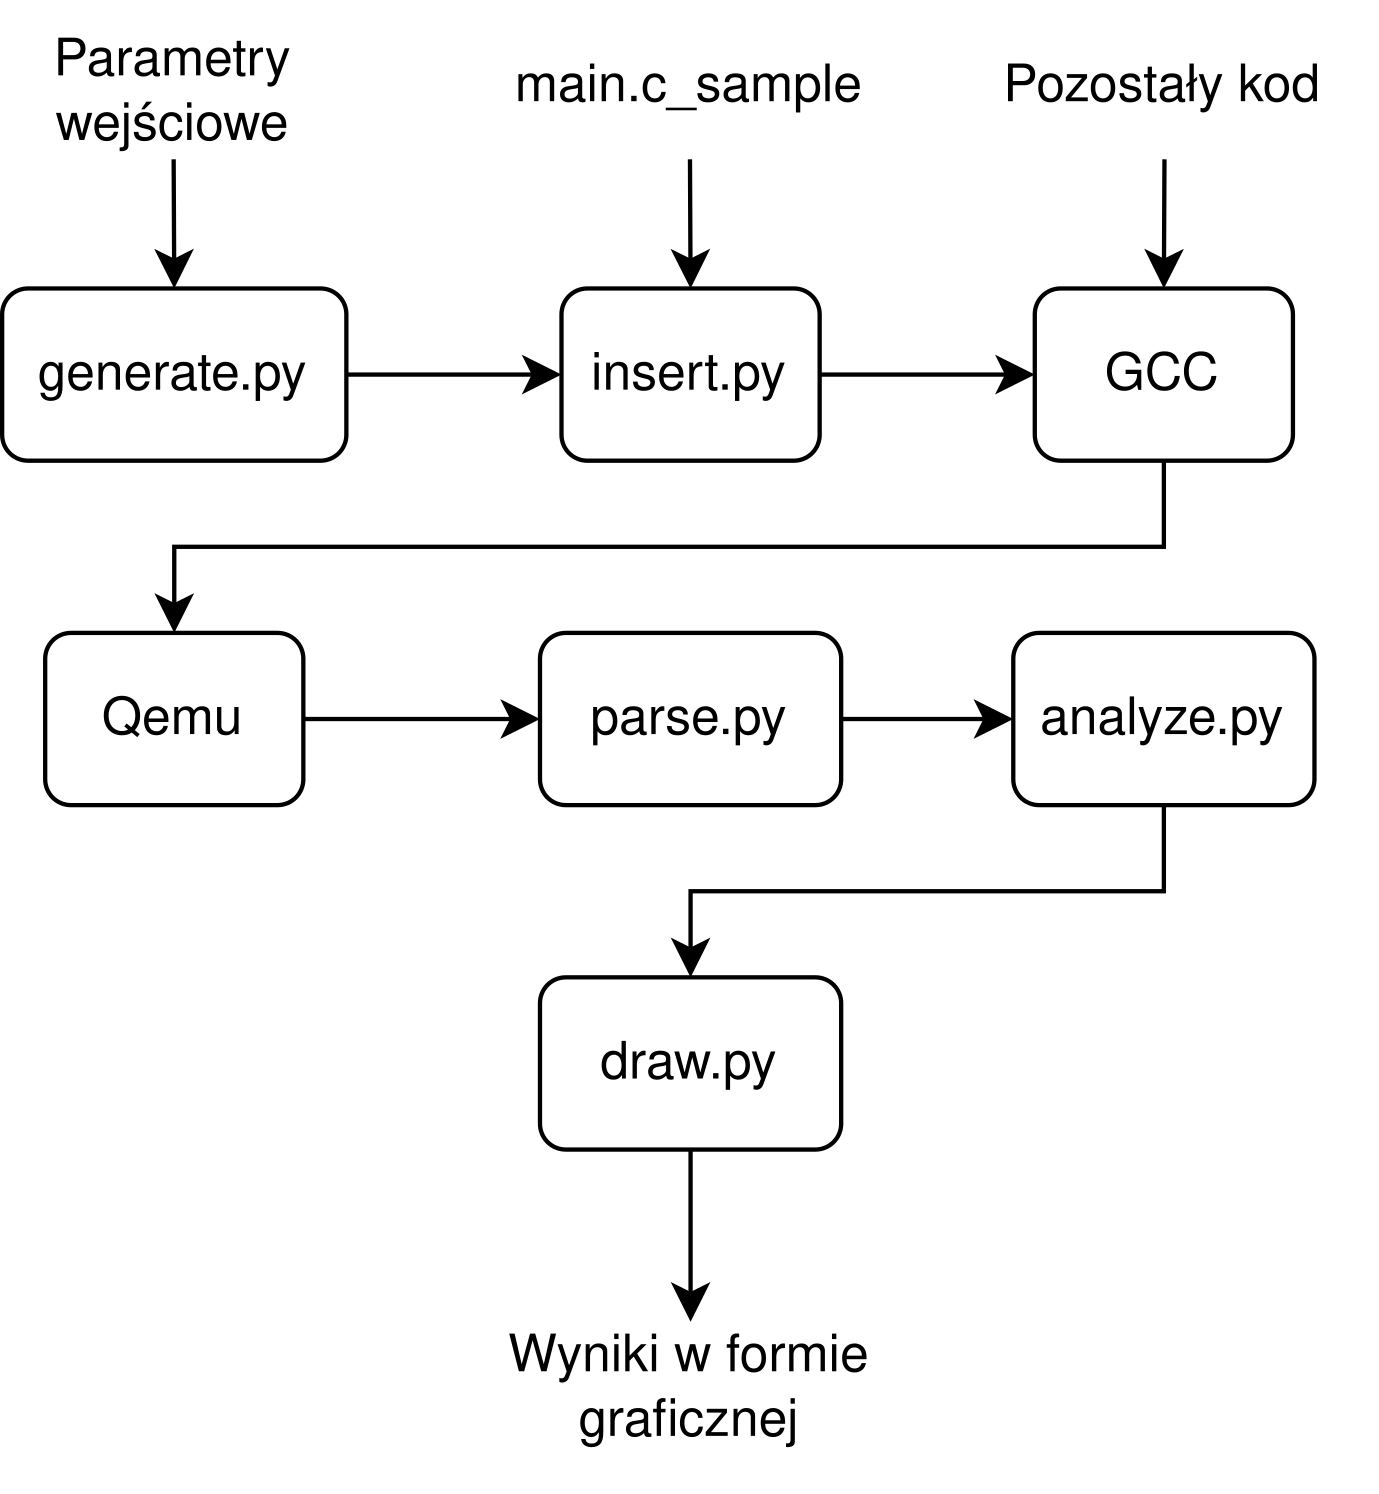
\includegraphics[width=0.7\textwidth]{Images/generate-parse-analyze.png}
    \caption{Zestaw narzędzi i połączenie z Qemu}
    \label{fig:generate-parse-analyze}
\end{figure}

Aby to przeanalizować, stworzono zestaw narzędzi w języku Python, który automatyzuje ten proces. Finalna architektura jest pokazana na \cref{fig:generate-parse-analyze}, gdzie każdy wątek odpowiada za:

\begin{itemize}
    \item \textit{generate.py}: generuje plik JSON zawierający metadane procesów.
    \item \textit{insert.py}: na podstawie metadanych procesów wygenerowanych w poprzednim tworzy funkcje w języku C (ponieważ każdy proces jest reprezentowany jako funkcja w FreeRTOS) z wykorzystaniem parametrów z wygenerowanego przez \textit{generate.py} pliku JSON. Następnie wygenerowane funkcje są wklejane do odpowiednio przygotowanego pliku \textit{main.c\_sample}, a otrzymany plik o nazwie \textit{main.c} jest zapisywany w systemie plików, gdzie on może zostać znaleziony przez kompilator.
    \item \gls{gcc}: otrzymuje \textit{main.c} oraz pozostały kod systemu operacyjnego, kompiluje, FreeRTOS przechodząc przez cały proces kompilacji programu w języku C, tzn. od etapu preprocesora do linkowania, tworząc plik binarny dla architektury \gls{arm}v7M. Plik ten jest zapisywany w systemie plików, gdzie on może być znaleziony przez Qemu.
    \item Qemu: odczytuje plik binarny i uruchamia go. Po uruchomieniu system operacyjny przechodzi przez proces inicjalizacji i zaczyna wykonywać wcześniej zdefiniowane procesy. W trakcie wykonywania Qemu zapisuje informacje o wykonywanych funkcjach systemowych do pliku tekstowego, który jest zapisywany w systemie plików, gdzie on może być znaleziony i przeanalizowany.
    \item \textit{parse.py}: otwiera i analizuje plik tekstowy zawierający informacje o wykonywanych funkcjach, zapisane wcześniej przez Qemu. Po analizie dane dotyczące każdego z procesów są zapisywane w pliku JSON w systemie plików. Zapisywane dane to: rozpoczęcie wykonywania każdego z procesów, zakończenie wykonywania każdego z procesów oraz liczba wywłaszczeń dla każdego z procesów.
    \item \textit{analyze.py}: odczytuje plik JSON otrzymany z poprzedniego kroku i oblicza następujące wskaźniki: liczbę sukcesów w osiągnięciu celu przed najgorszym czasem osiągnięcia celu dla każdego z procesów, liczbę porażek w osiągnięciu celu przed najgorszym czasem osiągnięcia celu dla każdego z procesów.
    \item \textit{draw.py}: tworzy wykresy na podstawie pliku JSON wygenerowanego w poprzednim kroku.
\end{itemize}

Każdy z elementów przedstawionych na \cref{fig:generate-parse-analyze} jest szczegółowo omówiony w dalszej części pracy.

\subsubsection{Problemy i założenia}

Podczas tworzenia wyżej przedstawionej listy narzędzi ujawniło się kilka problemów, które wpłynęły nie tylko na proces pomiaru i analizy, ale także na proces generowania metadanych procesów, jak również i na implementację algorytmów.

Wykorzystanie Qemu zamiast rzeczywistej płytki wprowadziło komplikacje, ponieważ Qemu jest emulatorem uruchamianym wewnątrz systemu operacyjnego użytkownika (w ramach tej pracy używano dystrybucji Linux'a o nazwie Ubuntu w wersji 22.04.1 na architekturze sprzętowej x86\_64) jako aplikacja. Oznacza to, że Qemu dzieli zasoby jednostki obliczeniowej użytkownika z innymi procesami, co sprawia, że w pewnym momencie Qemu może nie otrzymać czasu na wykonanie swoich instrukcji, co z kolei oznacza, że instrukcje Qemu nie są wykonywane w czasie rzeczywistym.

Z kolei, Qemu uruchamia wewnątrz siebie emulowaną platformę, na której działa badany system operacyjny. Skoro instrukcje Qemu nie są wykonywane w czasie rzeczywistym, emulowana platforma także nie działa w czasie rzeczywistym. Oznacza to, że jeżeli zegar systemowy emulowanej platformy został skonfigurowany na 50 MHz, to nie oznacza, że po uruchomieniu Qemu, rejestr przechowujący wartość zegara systemowego będzie modyfikowany z częstotliwością 50 MHz. Może to być dowolna inna częstotliwość, zależna od zasobów jednostki obliczeniowej użytkownika oraz od okresu, w jakim Qemu je otrzymuje. Może to nawet nie być periodyczne. Z tego wynika, że nie można mierzyć czas potrzebny na wykonanie czegokolwiek uruchamianego wewnątrz Qemu w sekundach ani częstości w hercach. W takim przypadku, w jaki sposób mierzyć i określać czas wykonywania procesów oraz momenty rozpoczęcia i zakończenia ich wykonywania?

Pierwszym pomysłem było użycie wartości zegara systemowego emulowanej przez Qemu architektury, czyli mierzenie wszystkich wielkości systemowych w różnicach pomiędzy wartościami zegara, które są dostępne w pewnym miejscu w pamięci. Jest to możliwe do zrobienia wewnątrz systemu (tzn. FreeRTOS może odczytywać wartości zegara), jak i z zewnątrz. Analiza ciągłego odczytu pamięci emulowanej architektury umożliwia też analizę wykonywanych działań w systemie, ponieważ oprócz rejestru ze stanem zegara w pamięci można znaleźć inne rejestry, np. wskaźnik na aktualnie używany przez emulowaną jednostkę obliczeniową stos, co pozwala na śledzenie wykonywanych procesów.

Byłoby to dobre rozwiązanie, gdyby nie problem, że Qemu nie emuluje mikroarchitekturę (tzn. właściwości sprzętowych), lecz tylko architekturę widzianą przez programistę systemowego i aplikacji. Oznacza to, że Qemu emuluje wykonywanie instrukcji dla określonej architektury (\gls{arm}v7M), ale nie emuluje, jak te instrukcje są wykonywane w odpowiedniej mikroarchitekturze.

Głównym problemem jest to, że nie wiadomo, ile okresów emulowanego zegara systemowego zajmie wykonywanie jednej instrukcji emulowanej architektury. Na przykład, dla Cortex M3 czas potrzebny na wykonanie instrukcji \textit{cmp} wynosi jeden okres zegara systemowego. Kiedy Cortex M3 jest emulowany przez Qemu, nie ma pewności, czy instrukcja \textit{cmp} zostanie wykonana w ciągu jednego okresu emulowanego zegara systemowego.

Uwzględniając powyższe, można wyciągnąć wniosek, że pomiar emulowanego zegara systemowego i porównywanie zdarzeń na podstawie tych pomiarów nie zawsze będzie sensowne. Ponieważ pomiędzy na przykład, dwoma periodycznymi wydarzeniami w systemie, rejestr zawierający wartość zegara systemowego może być zmodyfikowany o różne wartości, czasem wartość wzrośnie o jedną jednostkę, a innym razem to będzie inna jednostka.

Aby móc analizować efektywność używanych algorytmów, symulować czas potrzebny na osiągniecie celu przez proces oraz przeprowadzać pomiary, jako miarę czasu (czyli minimalny odcinek czasu) wybrano wartość zegara systemu operacyjnego, zwanego w FreeRTOS jako \textit{SysTick} (ang. System Tick). Nie jest istotne, ile realnego czasu minie pomiędzy chwilami, w których zegar systemu operacyjnego zmienia swój stan. Ważne jest, że ta zmiana się odbyła, a pomiędzy chwilami zmian stanu zegara wykonywane były inne operacje, które trwały dokładnie tyle czasu, ile minęło pomiędzy tymi dwoma zmianami stanu zegara systemu operacyjnego.

Czyli teraz czas wykonywania procesu będzie mierzony nie w sekundach lub ich ułamkach, lecz w okresach zegara systemu operacyjnego. Na przykład, można powiedzieć, że proces potrzebuje 100 okresów zegara systemu operacyjnego, aby osiągnąć swój cel albo, że proces jest periodyczny i pomiędzy dwoma momentami czasu, kiedy proces przechodzi do gotowości do wykonania, mija 500 okresów zegara systemu operacyjnego, i tak dalej. Jednostka, reprezentująca okres zegara systemu operacyjnego, w dalszej części pracy będzie nazywana \textit{SysTick}.

Owszem, takie założenie jest użyteczne, gdy nie jest ważne, ile dokładnie czasu minęło pomiędzy zmianami stanu zegara systemu operacyjnego.

Podczas pomiaru i analizy nie będzie uwzględniony czas wykonywania jakichkolwiek innych funkcji systemu operacyjnego, ponieważ: większość funkcji systemu operacyjnego została usunięta podczas kompilacji jako zbędne w ramach tej pracy, oraz dlatego, że celem tej pracy jest determinizm, a nie wydajność systemu. Uwzględniając powyższe założenia, można wyciągnąć wniosek, że wydajność końcowego systemu w ramach tej pracy nie wpłynie na analizę determinizmu, ponieważ jako miara czasu przyjęto fakt zmiany stanu zegara systemu operacyjnego, nie uwzględniając, ile realnego czasu minęło pomiędzy dwoma zmianami, ani ile czasu zajęła ta zmiana.

\subsubsection{Generacja parametrów, tworzenie procesów}

Generacja parametrów dla tworzenia procesów, jak zostało to opisane powyżej (\cref{fig:generate-parse-analyze}), odbywa się za pomocą skryptu \textit{generate.py}. Skrypt ten otrzymuje następujące parametry w formacie JSON (zamieszczone poniżej dane są przykładowe):

\begin{lstlisting}[caption={Parametry wejściowe do generacji}, label={lst:input-generation-parameters}]
{
    "TaskAmount": 10,
    "PriorityOverlapping": 0,
    "StdMeanPeriod": [1600,100],
    "LowUpPeriod": [2,30],
    "StdMeanDeadline": [1400,100],
    "LowUpDeadline": [2,1],
    "StdMeanExec": [20,10],
    "LowUpExec": [10,300],
    "StdMeanPriority": [126,250],
    "LowUpPriority": [1,251]
}
\end{lstlisting}

Gdzie:

\begin{itemize}
    \item \textit{TaskAmount}: liczba procesów.
    \item \textit{PriorityOverlapping}: flaga sygnalizująca, czy priorytety zdefiniowane dla procesów mogą się powtarzać.
    \item \textit{StdMeanPeriod}: parametry rozkładu normalnego (rozkładu Gaussa) używanego do generowania okresu gotowości do wykonywania procesów periodycznych. Pierwszy element tabeli to odchylenie standardowe, a drugi to wartość oczekiwana.
    \item \textit{LowUpPeriod}: ograniczenia dla wartości okresu, odpowiednio dolne i górne;
    \item \textit{StdMeanDeadline}: parametry rozkładu normalnego (rozkładu Gaussa) używanego do generowania najgorszego czasu osiągnięcia celu przez proces. Pierwszy element tabeli to odchylenie standardowe, a drugi to wartość oczekiwana.
    \item \textit{LowUpDeadline}: ograniczenia dla wartości najgorszego czasu osiągnięcia celu przez proces, odpowiednio dolne i górne.
    \item \textit{StdMeanExec}: parametry rozkładu normalnego (rozkładu Gaussa) używanego do generowania czasu potrzebnego procesowi na osiągnięcie swojego celu. Pierwszy element tabeli to odchylenie standardowe, a drugi to wartość oczekiwana.
    \item \textit{LowUpExec}: ograniczenia dla wartości czasu potrzebnego procesowi na osiągnięcie swojego celu, odpowiednio dolne i górne.
    \item \textit{StdMeanPriority}: parametry rozkładu normalnego (rozkładu Gaussa) używanego do generowania priorytetu przypisywanego każdemu procesowi. Pierwszy element tabeli to odchylenie standardowe, a drugi to wartość oczekiwana.
    \item \textit{LowUpPriority}: ograniczenia dla wartości priorytetu, odpowiednio dolne i górne.
\end{itemize}

Rozkłady prawdopodobieństwa zostały wybrane do generowania parametrów procesów w celu przybliżenia do rozkładu parametrów w rzeczywistych sytuacjach. Oznacza to, że w rzeczywistości procesy nie mogą mieć identycznych lub bardzo podobnych parametrów, tylko ich wartości są rozproszone na określonym przedziale. Zadaniem rozkładów prawdopodobieństwa jest symulacja tej niejednorodności.

Wszystkie wymienione powyżej parametry są dobierane ręcznie w celu zasymulowania przybliżonego do rzeczywistości przypadku. Na przykład, można wygenerować zestaw parametrów procesów, w którym w systemie będzie występowała duża liczba procesów o niskich priorytetach oraz długie procesy o wyższych priorytetach, a następnie przekazać te dane do Qemu, aby sprawdzić pewny algorytm w takich warunkach.

Wygenerowane dane są zapisywane w formacie JSON w następującej postaci (przykład dla jednego procesu):

\begin{lstlisting}[caption={Wygenerowane parametry procesu}, label={lst:proces-parameters-generated}]
{
    "v1_Task": {
        "TaskName": "v1_Task",
        "TaskPriority": 57,
        "TaskExecutionTime": 13,
        "TaskDeadline": 30,
        "TaskPeriod": 106
    }
}
\end{lstlisting}

Gdzie:

\begin{itemize}
    \item \textit{TaskName}: nazwa procesu.
    \item \textit{TaskPriority}: priorytet procesu.
    \item \textit{TaskExecutionTime}: czas potrzebny procesowi na osiągnięcie celu, jednostka - \textit{SysTick}.
    \item \textit{TaskDeadline}: najgorszy czas osiągnięcia celu przez proces, jednostka - \textit{SysTick}.
    \item \textit{TaskPeriod}: okres gotowości do wykonywania procesu, jednostka - \textit{SysTick}.
\end{itemize}

Te dane są interpretowane przez skrypt \textit{insert.py}, który generuje kod w języku C i wkleja go do wspomnianego wyżej (\cref{fig:generate-parse-analyze}) pliku \textit{main.c\_sample}. Na przykładzie \ref{lst:c-generated} pokazano wygenerowany kod w języku C dla danych z przykładu \ref{lst:proces-parameters-generated}:

\begin{lstlisting}[language=C, caption={Wygenerowany kod w języku C}, label={lst:c-generated}]
void v1_Task(void *pvParameters);

int main(void){
  xTaskCreate(v1_Task, "v1_Task", TASK_STACK_LENGHT_WORDS, NULL, 57, 13, 30, NULL);

  vTaskStartScheduler();
  while(1){};
}

void v1_Task (void *pvParameters){
  TickType_t xLastWakeTime = 0;

  while (1){
    pxCurrentTCB->xTaskCurrentExecutionTime = pxCurrentTCB->xTaskExecutionTime;
    do{}while( pxCurrentTCB->xTaskCurrentExecutionTime != 0 );

    vTaskDelayUntil(&xLastWakeTime, 106);
    }
    vTaskDelete(NULL);
}
\end{lstlisting}

A więc wygenerowany został prototyp funkcji reprezentującej proces, polecenie tworzenia procesu w systemie operacyjnym za pomocą funkcji \textit{xTaskCreate} i procesu w postaci definicji funkcji \textit{v1\_Task}. Należy również zauważyć, że jest to część wygenerowanego pliku, obcięta w celu prezentacji przykładu. Nie zawiera ona wszystkich definicji i poleceń.

\subsubsection{Kompilacja i wybór algorytmów}

Kompilacja systemu operacyjnego była przeprowadzona za pomocą narzędzi Make i \gls{gcc}. Narzędzie Make organizuje cały kod źródłowy w jeden projekt i przekazuje go do narzędzi \gls{gcc}.

Wśród zbieranego przez Make kodu źródłowego znajduje się plik \textit{FreeRTOS.h}, który zawiera definicje preprocesora języka C konfigurujące FreeRTOS. W pliku tym dodano także definicje umożliwiające wybór używanego algorytmu.

\subsubsection{Sposób zbierania danych o procesach}

Zgodnie z założeniem opisanym powyżej, wszystkie operacje w systemie są mierzone w okresach zegara systemu operacyjnego (czyli FreeRTOS). Pozostaje jedynie znaleźć sposób, w jaki można mierzyć te okresy oraz wydarzenia spowodowane zmianami wartości zegara systemowego.

Jak już wspomniano, do tego celu można wykorzystać możliwość odczytywania pomięci emulowanego systemu i późniejszej jej analizy. Ten sposób został uznany przez autora za zbyt skomplikowany. Jako alternatywę zdecydowano skorzystać z funkcji Qemu, która pokazuje, które funkcje są wykonywane w danym momencie w emulowanym systemie. Przykład:

\begin{lstlisting}[language=C, caption={Przykładowe logi z Qemu}, label={lst:qemu-example-logs}]
Stopped execution of TB chain before 0x7df2b4031880 v1_Task
Trace 0: 0x7df2b401e280 SysTick_Handler
Trace 0: 0x7df2b401e480 SysTick_Handler
Trace 0: 0x7df2b401e700 xTaskIncrementTick
Trace 0: 0x7df2b401f200 xTaskIncrementTick
Trace 0: 0x7df2b401f980 SysTick_Handler
Trace 0: 0x7df2b40200c0 SysTick_Handler
Trace 0: 0x7df2b4031880 v1_Task
Stopped execution of TB chain before 0x7df2b4031880 v1_Task
Trace 0: 0x7df2b401e280 SysTick_Handler
Trace 0: 0x7df2b401e480 SysTick_Handler
Trace 0: 0x7df2b401e700 xTaskIncrementTick
Trace 0: 0x7df2b401f200 xTaskIncrementTick
Trace 0: 0x7df2b401f980 SysTick_Handler
Trace 0: 0x7df2b40200c0 SysTick_Handler
Trace 0: 0x7df2b4031880 v1_Task
\end{lstlisting}

Jest to fragment logów wykonywania funkcji FreeRTOS z Qemu. Widać tu funkcje: \textit{v1\_Task}, \textit{SysTick\_Handler} i \textit{xTaskIncrementTick}. Pierwsza funkcja jest jednym z procesów zdefiniowanych przed uruchomieniem systemu, zaś ostatnie dwie są funkcjami jądra FreeRTOS, odpowiadającymi za modyfikację wartości zegara systemu operacyjnego.

Mając wiedzę o tych funkcjach i o kolejności ich wykonywania, można wywnioskować, co jest robione w danym momencie w systemie operacyjnym. Na przykład w powyższym przykładzie przedstawiono dwa momenty zmiany stanu zegara systemu operacyjnego, wraz z procesem, który jest wykonywany pomiędzy tymi zmianami.

Za pomocą tej wiedzy można stworzyć listę reguł opisujących pewne działania podejmowane przez system operacyjny. Ponieważ logi te są dość obszerne, zdecydowano napisać skrypt w języku Python, który automatycznie analizuje logi, wykorzystując te reguły do wykrywania potrzebnych dla analizy procesów zachodzących wewnątrz systemu operacyjnego. Jak wspomniano wcześniej (\cref{fig:generate-parse-analyze}), skrypt ten nazywa się \textit{parse.py}.

W tym skrypcie były zdefiniowane reguły, na podstawie których można wykryć następujące wydarzenia:

\begin{itemize}
    \item Moment, w którym proces po raz pierwszy pojawia się w systemie.
    \item Moment, w którym proces ponownie zaczyna swoje wykonywanie.
    \item Moment, w którym proces zostaje wywłaszczony przez inny proces.
    \item Moment, w którym proces kontynuuje wykonywanie po wywłaszczeniu.
    \item Moment, w którym proces kończy wykonywanie.
    \item Moment, w którym modyfikowana jest wartość zegara systemu operacyjnego.
\end{itemize}

Skrypt zapisuje, przy jakiej wartości zegara systemu operacyjnego te wydarzenia występują. Wartość zegara jest obliczana również na podstawie rejestrowanej działalności systemu operacyjnego, zgodnie z przykładem powyżej. Przykład zapisanych danych w formacie JSON w przypadku wykonywania jednego procesu:

\begin{lstlisting}[caption={Przykładowe pomiary dla jednego procesu}, label={lst:example-process-measurements}]
"v1_Task": {
    "TaskName": "v1_Task",
    "TaskStart": [8,44],
    "TaskEnd": [11,47],
    "TaskPreemptedTimes": 0
},
\end{lstlisting}

Gdzie:

\begin{itemize}
    \item \textit{TaskName}: zawiera nazwę procesu.
    \item \textit{TaskStart}: tabela zawierająca stany zegara systemu operacyjnego, kiedy proces rozpoczął swoje wykonywanie, jednostka - \textit{SysTick}.
    \item \textit{TaskEnd}: tabela zawierająca stany zegara, kiedy proces zakończył swoje wykonanie, jednostka - \textit{SysTick}.
    \item \textit{TaskPreemptedTimes}: liczba razy, kiedy proces został wywłaszczony w analizowanym odcinku czasu.
\end{itemize}

\subsubsection{Analiza i wyniki w postaci graficznej}

Dane uzyskane ze skryptu \textit{parse.py} są przekazywane do skryptu \textit{analyze.py}, który je analizuje i generuje niezbędne dane do opisu zachowania procesów w analizowanym odcinku. Poniżej znajdują się przykładowe dane dla przypadku z czterema procesami:

\begin{lstlisting}[caption={Przykładowe wyniki analizy dla czterech procesów}, label={lst:example-process-analisys}]
{
    "MetDeadline": {
        "v3_Task": 5,
        "v2_Task": 3,
        "v4_Task": 4,
        "v1_Task": 2
    },
    "MissDeadline": {
        "v3_Task": 0,
        "v2_Task": 0,
        "v4_Task": 0,
        "v1_Task": 0
    },
    "LoadFactor": 0.5951709401709402,
    "MeanTaskExecutionTime": 2.75
}
\end{lstlisting}

Gdzie:

\begin{itemize}
    \item \textit{MetDeadline}: lista procesów oraz wartości, które pokazują, ile razy w badanym przypadku każdy z procesów osiągnął swój cel, spełniając ograniczenia czasowe; ten parametr nie ma jednostek.
    \item \textit{MissDeadline}: lista procesów oraz wartości, które pokazują, ile razy w badanym przypadku każdy z procesów osiągnął swoją cel, nie spełniając ograniczeń czasowych; ten parametr nie ma jednostek.
    \item \textit{LoadFactor}: obciążenie systemu dla analizowanego przypadku; ten parametr nie ma jednostek.
    \item \textit{MeanTaskExecutionTime}: średni czas potrzebny procesowi na osiągnięcie swojego celu, mierzony w jednostkach zegara systemu operacyjnego. 
\end{itemize}

Oprócz danych otrzymanych z poprzedniego kroku \textit{analyze.py} potrzebuje także danych wygenerowanych przez skrypt \textit{generate.py}. \cref{alg:timings-algorithm} przedstawia algorytm obliczenia spełnienia ograniczeń czasowych (czyli \textit{MetDeadline} i \textit{MissDeadline}) na podstawie danych uzyskanych ze skryptów \textit{parse.py} i \textit{analyze.py}.

\begin{algorithm}
\caption{Algorytm liczący spełnienie ograniczeń czasowych dla każdego z procesów}\label{alg:timings-algorithm}
\begin{algorithmic}[1]
\For {proces \textbf{in} lista procesów}
  \State \textit{MetDeadline}[proces]=0
  \State \textit{MissDeadline}[proces]=0
  \ForAll {indeks \textbf{in} oblicz rozmiar \textit{TaskEnd}[proces]}
    \State czas gotowości do wykonywania = indeks * \textit{TaskPeriod}[proces]
    \State najgorszy czas osiągnięcia celu = czas gotowości do wykonywania + \textit{TaskDeadline}[proces]
    \If {\textit{TaskEnd}[proces] <= najgorszy czas osiągnięcia celu}
      \State \textit{MetDeadline}[proces] = \textit{MetDeadline}[proces] + 1
    \ElsIf {\textit{TaskEnd}[proces] > najgorszy czas osiągnięcia celu}
      \State \textit{MissDeadline}[proces] = \textit{MissDeadline}[proces] + 1
    \EndIf
  \EndFor
\EndFor
\end{algorithmic}
\end{algorithm}

Natomiast obciążenie systemu (ang. utilization factor) oblicza sie według następującej formuły:

\large
\begin{equation}
    U = \sum_{i=1}^{n} \frac{T_{ex\_i}}{T_{ready\_i}}
    \label{eq:utilization}
\end{equation}
\normalsize

Gdzie: $U$ - współczynnik obciążenia systemu; $n$ - liczba procesów, $T_{ex\_i}$ - czas potrzebny  procesowi na osiągnięcie celu, jednostka: \textit{SysTick}; $T_{ready\_i}$ - czas,
kiedy każdy proces jest przypisywany do listy \textit{pxReadyTasksLists}, jednostka: \textit{SysTick}.

Średni czas potrzebny procesowi na osiągnięcie celu oblicza się zgodnie z następującą formułą:

\large
\begin{equation}
    T_{exav}= \frac{1}{n}\sum_{i=1}^nT_{ex\_i}
    \label{eq:avarage-ex-time}
\end{equation}
\normalsize

Gdzie: $T_{exav}$ - średni czas potrzebny procesowi na osiągnięcie celu, jednostka: \textit{SysTick}; $n$ - liczba procesów;  $T_{ex\_i}$ - czas potrzebny każdemu procesowi na osiągnięcie celu, jednostka: \textit{SysTick}.

Następnie skrypt \textit{draw.py} zbiera dane od skryptu \textit{analyze.py} i generuje wykresy na ich podstawie danych.

\subsection{Implementacja wybranych algorytmów w FreeRTOS}

W tej części pracy omówione zostaną wybrane algorytmy zarządzania zasobami jednostki obliczeniowej oraz ich implementacja w FreeRTOS.

\subsubsection{Standardowe algorytmy w FreeRTOS}

FreeRTOS ma jeden standardowy algorytm, który posiada trzy odmiany. Algorytm ten nazywa się HPF (ang. Highest Priority First). Zasada jego działania jest następująca: zasoby jednostki obliczeniowej jako pierwszy otrzymuje proces o największym statycznie zdefiniowanym priorytecie. Priorytet jest definiowany przez użytkownika przy programowaniu systemu i nie zmienia się w trakcie jego działania.

Początkowo ten algorytm nie wykorzystuje wywłaszczania, ale wywłaszczanie można włączyć, dodając do pliku \textit{FreeRTOSConfig.h} definicję preprocesora \textit{configUSE\_PREEMPTION} z wartością \textit{1}. To jest druga odmiana algorytmu. Trzecią odmianą jest dodanie współdzielenia czasu przez procesy o tym samym priorytecie. Jest to możliwe po dodaniu do pliku \textit{FreeRTOSConfig.h} definicji preprocesora \textit{configUSE\_TIME\_SLICING} o wartości \textit{1}.

\subsubsection{Kluczowe pojęcia w FreeRTOS}

Metadane każdego procesu w FreeRTOS są przechowywane w strukturach zwanych \gls{tcb}. Na przykładzie \ref{lst:freertos-tcb} przedstawiony jest \gls{tcb} używany podczas pracy przed wprowadzeniem modyfikacji.

\begin{lstlisting}[language=C, label={lst:freertos-tcb}, caption={Przykładowy TCB przed zmianami}]
typedef struct tskTaskControlBlock
{
    volatile StackType_t * pxTopOfStack;
    ListItem_t xStateListItem;
    ListItem_t xEventListItem;
    UBaseType_t uxPriority;
    StackType_t * pxStack;
    char pcTaskName[ ( 10 ) ];
} tskTCB;
\end{lstlisting}

Gdzie:

\begin{itemize}
    \item \textit{pxTopOfStack}: wskaźnik na ostatni element w stosie procesu, potrzebny dla dyspozytora.
    \item \textit{xStateListItem}: lista, do której proces jest aktualnie przypisany. Może to być lista procesów uśpionych (\textit{pxDelayedTaskList}) lub lista procesów gotowych do wykonania (\textit{pxReadyTasksLists}). W zależności od listy, do której jest przypisany proces, można wnioskować o stanie tego procesu, tj. czy jest uśpiony, czy gotowy do wykonywania.
    \item \textit{xEventListItem}: podstawowa funkcjonalność FreeRTOS, która nie jest używana w tej prace, a więc nie będzie tu opisana.
    \item \textit{uxPriority}: zmienna przechowująca priorytet procesu.
    \item \textit{pxStack}: wskaźnik na stos procesu.
    \item \textit{pcTaskName}: tabela z nazwą procesu. 
\end{itemize}

Struktura pokazana na przykładzie \ref{lst:freertos-tcb} przeszła już przez preprocesor języka C, więc jest pozbawiona wszystkich zbędnych elementów, które są niepotrzebnych w ramach tej pracy.

Proces jest tworzony jako funkcja w języku C (przykład \ref{lst:c-generated}), i rejestrowany w systemie za pomocą funkcji \textit{xTaskCreate}. Po zarejestrowaniu wszystkich procesów w systemie uruchamiany jest nadzorca systemu operacyjnego za pomocą funkcji \textit{vTaskStartScheduler}. Podczas uruchomienia nadzorcy, tworzony jest tzw. proces zerowy, który jest wykonywany, gdy żaden inny proces nie jest gotowy do wykonania. W trakcie pracy systemu procesom są przydzielane zasoby jednostki obliczeniowej zgodnie z zasadami zdefiniowanymi przez planistę.

Podczas wykonywania procesy zmieniają swoje stany. W trakcie tej pracy będą używane tylko dwa stany procesu: gotowy do wykonywania i uśpiony. Stany te są definiowane poprzez przepisanie procesu do odpowiedniej listy, tj. \textit{pxReadyTasksLists} i \textit{pxDelayedTaskList}. Te listy są strukturami w języku C. Ich dokładny opis nie jest potrzebny, ponieważ nie będą one modyfikowane w ramach tej pracy.

Podczas pracy FreeRTOS przechowuje wskaźnik na \gls{tcb} aktualnie wykonywanego procesu w globalnej zmiennej \textit{pxCurrentTCB}.

\subsubsection{Problemy i założenia}

Napotkane problemy:

\begin{itemize}
    \item Problem z priorytetami w FreeRTOS.
    \item Problem z symulacją czasu wykonywania procesu.
    \item Problem z metadanymi procesów.
\end{itemize}

W tej prace wybrane do integracji w FreeRTOS algorytmy zarządzania zasobami jednostki obliczeniowej posiadają różne właściwości. Problemem jest to, że FreeRTOS został zbudowany w sposób, który ściśle wiąże cały kod systemu operacyjnego z algorytmem, a dokładniej ze sposobem definiowania, zarządzania i używania priorytetów procesów. Priorytety te są używane wszędzie w kodzie FreeRTOS, a co najważniejsze, listy, do których są przepisywane wskaźniki na \gls{tcb} (czyli \textit{pxReadyTasksLists} i \textit{pxDelayedTaskList}), także wykorzystują priorytety.

Struktura kodu systemu operacyjnego, która używa pewnych danych systemowych do definiowania większości obiektów systemu, ma sens, gdy te dane są definiowane przed definiowaniem tych pozostałych obiektów systemu.

Jest to dobre rozwiązanie dla standardowego algorytmu używanego w FreeRTOS, ponieważ w takim przypadku priorytety, które są używane do definiowania większości obiektów w FreeRTOS, są definiowane przez użytkownika na etapie programowania. Natomiast w ramach tej pracy będą implementowane algorytmy, które nie używają priorytetów (np. FCFS), lub algorytmy używające priorytetów dynamicznych.

Aby zaimplementować te algorytmy, wprowadzono modyfikacje dostosowujące FreeRTOS do przypadków, gdy priorytety są dynamiczne lub nie są używane w ogóle. Aktywacja tych modyfikacji i przywrócenie standardowego kodu jest możliwa za pomocą manipulacji definicją preprocesora języka C o nazwie \textit{USE\_FREERTOS\_CLASSIC\_SCHEDULER} w pliku \textit{FreeRTOSConfig.h}.

Podczas badań potrzebny był również sposób na symulację czasu, który proces potrzebuje na osiągnięcie swojego celu. Ponieważ w ramach tego zadania analizowana będzie wydajność algorytmów, cel procesu nie jest istotny, jak również nie ma znaczenia, w jaki sposób każdy z procesów będzie ten cel osiągał. Ważne jest natomiast, aby można było łatwo i dokładnie określić, ile czasu potrzebuje proces na osiągnięcie swojego celu.

Uwzględniając powyższe, zdecydowano symulować wykonywanie procesu za pomocą pętli. Na przykładzie \ref{rst:process-structure-example} pokazano wybraną strukturę procesu.

\begin{lstlisting}[language=C, label={rst:process-structure-example}, caption={Używana struktura procesu}]
void v1_Task (void *pvParameters){
  TickType_t xLastWakeTime = 0;

  while (1){
    pxCurrentTCB->xTaskCurrentExecutionTime = pxCurrentTCB->xTaskExecutionTime;
    do{}while( pxCurrentTCB->xTaskCurrentExecutionTime != 0 );

    vTaskDelayUntil(&xLastWakeTime, 106);
  }

  vTaskDelete(NULL);
}
\end{lstlisting}

Gdzie:

\begin{itemize}
    \item \textit{v1\_Task}: przykładowa nazwa procesu.
    \item \textit{pvParameters}: parametry, które mogą być przekazane procesowi. Nie są one wykorzystywane w tej prace i nie będą tu omówione.
    \item \textit{xLastWakeTime}: zmienna potrzebna dla periodycznego uśpienia procesu po osiągnięciu celu.
    \item \textit{xTaskCurrentExecutionTime}: zmienna przechowująca czas, którego proces potrzebuje do osiągnięcia celu, zmniejszana o jeden przy każdej zmianie stanu zegara systemu operacyjnego.
    \item \textit{xTaskExecutionTime}: czas, który proces potrzebuje na osiągnięcie celu od początku, jest statycznie definiowany i niezmieniany podczas wykonywania.
    \item \textit{vTaskDelayUntil}: funkcja powodująca uśpienie procesu na zdefiniowany okres, w tym przypadku 106 SysTick. Ten okres jest okresem gotowości procesu do wykonywania, znanym także jako \textit{TaskPeriod} (było to przedstawione na przykładzie \ref{lst:proces-parameters-generated}).
    \item \textit{vTaskDelete}: funkcja, która teoretycznie nigdy nie musi wykonać się. Jest częścią struktury procesu zgodnie z wymogami FreeRTOS i nie będzie tu opisana.
\end{itemize}

Jak widać z przykładu \ref{rst:process-structure-example}, proces wykonuje się, dopóki czas potrzebny na jego wykonanie (zdefiniowany statycznie przed uruchomieniem systemu poprzez zmienną \textit{xTaskExecutionTime}) nie upłynie (co jest sygnalizowane przez porównanie zmiennej \textit{xTaskCurrentExecutionTime} do zera). Podczas wykonywania proces znajduje się w pustej pętli i niczego nie robi. Wartość zmiennej \textit{xTaskExecutionTime} jest generowana przez skrypt \textit{generate.py} (czyli jest to \textit{TaskExecutionTime} z przykładu \ref{lst:proces-parameters-generated}), zaś wartość zmiennej \textit{xTaskCurrentExecutionTime} jest dynamicznie definiowana podczas rejestrowania procesu, oraz, jak widać na przykładzie \ref{rst:process-structure-example}, kiedy proces wychodzi z uśpienia (czyli funkcja \textit{vTaskDelayUntil} kończy swoje wykonywanie).

Należy również zauważyć, że zmienna \textit{pxCurrentTCB} nie powinna być udostępniana procesom i powinna być dostępna tylko dla jądra systemu operacyjnego. Natomiast w ramach tej pracy pominięto kwestie bezpieczeństwa i standardów napisania kodu, aby w krótszym casie zaimplementować potrzebne algorytmy i przeprowadzić potrzebne badania. Zresztą, te kwestie nie są w zakresie tej pracy, więc można je pominąć.

Jak widać na przykładzie \ref{rst:process-structure-example}, do \gls{tcb} zostały dodane nowe elementy pozwalające na symulację czasu potrzebnego procesowi na osiągnięcie swojego celu, są to zmienne \textit{xTaskCurrentExecutionTime} i \textit{xTaskExecutionTime}.

Oprócz tych dwóch nowych elementów, dodano także kilka innych elementów, potrzebnych do implementacji niektórych algorytmów. Nowy \gls{tcb}, który był wykorzystywany w ramach tej pracy, jest pokazany na przykładzie \ref{rst:new-tcb}

\begin{lstlisting}[language=C, label={rst:new-tcb}, caption={Zmodyfikowany \gls{tcb}}]
typedef struct tskTaskControlBlock
{
    volatile StackType_t * pxTopOfStack;
    ListItem_t xStateListItem;
    ListItem_t xEventListItem;
    StackType_t * pxStack;
    TickType_t xTaskStarted;
    TickType_t xTaskTimeExecuted;
    TickType_t xTaskExecutionTime;
    TickType_t xTaskCurrentExecutionTime;
    TickType_t xTaskExecutionPeriod;
    TickType_t xTaskExecutionDeadline;
    char pcTaskName[ ( 10 ) ];
} tskTCB;
\end{lstlisting}

Gdzie nowe elementy (w porównaniu do przykładu \ref{rst:process-structure-example}):

\begin{itemize}
    \item \textit{xTaskStarted}: przechowuje wartość zegara systemu operacyjnego, kiedy proces został przypisany do listy procesów gotowych do wykonywania.
    \item \textit{xTaskTimeExecuted}: przechowuje liczbę zmian stanu zegara systemu operacyjnego od momentu, kiedy proces zaczął wykonywanie. W przypadku, gdy proces zaczął wykonywanie, a następnie został wywłaszczony przez inny proces, logowanie czasu do tej zmiennej jest wstrzymywane do momentu, kiedy proces powróci do wykonania po wywłaszczeniu.
    \item \textit{xTaskExecutionTime}: wyjaśnione w przykładzie \ref{rst:process-structure-example}.
    \item \textit{xTaskCurrentExecutionTime}: wyjaśnione w przykładzie \ref{rst:process-structure-example}.
    \item \textit{xTaskExecutionPeriod}: okres gotowości procesu do wykonywania, generowany przez skrypt \textit{generate.py} (zgodnie z \ref{lst:proces-parameters-generated} to jest \textit{TaskPeriod}).
    \item \textit{xTaskExecutionDeadline}: najgorszy czas osiągnięcia celu przez proces, generowany przez skrypt \textit{generate.py} (zgodnie z \ref{lst:proces-parameters-generated} to jest \textit{TaskDeadline}).
\end{itemize}

Niektóre z tych nowych elementów są inicjalizowane statycznie podczas rejestrowania procesu, a inne są modyfikowane podczas pracy systemu.

\subsubsection{Sposób integracji nowych algorytmów}

Poprzednio pokazano (\cref{fig:cpu-resources-mult}), że za zarządzanie zasobami jednostki obliczeniowej w systemie operacyjnym jest odpowiedzialny jeden moduł, zwany także nadzorcą. Następnie nadzorca był podzielony (\cref{fig:armv8-m-context-switch}) na dyspozytora i planistę.

Jednak w rzeczywistości funkcje planisty i dyspozytora pełni nie jedna funkcja, a moduł ten nie jest umieszczony w jednym konkretnym miejscu w kodzie systemu operacyjnego, tylko jest to kod rozrzucony po całym systemie, który jednak można podzielić na części i wyodrębnić. Podział taki będzie specyficzny dla każdego systemu operacyjnego, ponieważ zależy od jego implementacji.

Natomiast w FreeRTOS planista może zostać podzielony na następujące części:

\begin{enumerate}
    \item Kod, który jest wykonywany przy rejestracji procesu w systemie. W FreeRTOS ten kod znajduje się wewnątrz funkcji \textit{prvAddNewTaskToReadyList}.
    \item Kod, który jest wykonywany w pewnych przypadkach powodujących przełączenie kontekstu. W FreeRTOS ten kod znajduje się wewnątrz funkcji \textit{vTaskSwitchContext}.
    \item Kod, który jest wykonywany periodycznie. W FreeRTOS ten kod znajduje się wewnątrz \textit{xTaskIncrementTick}.
\end{enumerate}

To, który z tych punktów trzeba zaimplementować, zależy od algorytmu. Punkt drugi jest jednak zawsze obowiązkowy. Na przykład punkt trzeci pewnie będzie potrzebny algorytmom, które odwołują się do planisty przy każdej zmianie wartości zegara systemowego, niezależnie od tego, czy wystąpiło zdarzenie powodujące zmianę kontekstu (np. algorytmy DARTS i RR tego potrzebują).

Wyjaśnienia implementacji poszczególnych algorytmów w dalszej części pracy będą odwoływać się do tych trzech punktów.

\subsubsection{FCFS}

\cref{alg:fcfs-algorithm} demonstruje algorytm FCFS w postaci pseudokodu. 

\begin{algorithm}[ht]
\caption{Pseudokod algorytmu FCFS}\label{alg:fcfs-algorithm}
\begin{algorithmic}[1]
\State pxCurrentTCB = Wybierz pierwszy proces z listy(\textit{pxReadyTasksLists})
\end{algorithmic}
\end{algorithm}

W tym przykładzie widać nazwy napisane bez spacji oraz nazwy napisane kursywą. Tu i w dalszej części pracy nazwy napisane bez spacji będą oznaczać zmienne, natomiast nazwy napisane bez spacji z użyciem kursywy będą oznaczać zmienne istniejące w kodzie systemu operacyjnego.

Potrzebne modyfikacje jądra FreeRTOS:

\begin{enumerate}
    \item Wybranie pierwszego zarejestrowanego procesu jako pierwszego procesu gotowego do wykonywania jeszcze przed uruchomieniem nadzorcy, czyli wewnątrz funkcji \textit{prvAddNewTaskToReadyList}.
    \item Wybranie pierwszego procesu z kolejki \textit{pxReadyTasksLists} do wykonania w momencie, gdy aktualny proces osiąga swój cel i jednostka obliczeniowa zostaje zwolniona, czyli potrzebna była modyfikacja funkcji \textit{vTaskSwitchContext}.
    \item Każdy proces zmieniający swój stan na stan gotowy do wykonywania musi być dodany do końca listy \textit{pxReadyTasksLists}.
\end{enumerate}

W standardowej implementacji FreeRTOS wszystkie procesysą dodawane na koniec listy \textit{pxReadyTasksLists}, więc implementacja trzeciego punktu nie była potrzebna.

\subsubsection{SJF}

\cref{alg:sjf-algorithm} demonstruje pseudokod algorytmu SJF.

\begin{algorithm}
\caption{Pseudokod algorytmu SJF}\label{alg:sjf-algorithm}
\begin{algorithmic}[1]
\ForAll {procesTCB \textbf{in} \textit{pxReadyTasksLists}}
    \If {procesTCB.\textit{xTaskExecutionTime} < \textit{pxCurrentTCB}.\textit{xTaskExecutionTime} }
        \State \textit{pxCurrentTCB}=procesTCB
    \EndIf
\EndFor
\end{algorithmic}
\end{algorithm}

Potrzebne modyfikacje jądra FreeRTOS:

\begin{enumerate}
    \item Modyfikacja funkcji \textit{prvAddNewTaskToReadyList}, aby przed uruchomieniem nadzorcy wybrany został do wykonania proces zgodnie z algorytmem SJF.
    \item Modyfikacja funkcji \textit{vTaskSwitchContext} aby przy każdym wywołaniu planisty zasoby jednostki obliczeniowej były przedzielane procesowi zgodnie z algorytmem SJF.
\end{enumerate}

\subsubsection{SRTN}

\cref{alg:srtn-algorithm} demonstruje pseudokod algorytmu SRTN.

\begin{algorithm}
\caption{Pseudokod algorytmu SRTN}\label{alg:srtn-algorithm}
\begin{algorithmic}[1]
\ForAll {procesTCB \textbf{in} \textit{pxReadyTasksLists}}
    \State procesTCB.RemainingExecutionTime = Oblicz RemaningExecutionTime dla procesu(procesTCB)
    \State \textit{pxCurrentTCB}.RemainingExecutionTime = Oblicz RemaningExecutionTime dla procesu(\textit{pxCurrentTCB})
    \If {procesTCB.RemainingExecutionTime < \textit{pxCurrentTCB}.RemainingExecutionTime }
        \State \textit{pxCurrentTCB}=procesTCB
    \EndIf
\EndFor
\end{algorithmic}
\end{algorithm}

\textit{RemaningExecutionTime} z tego przykładu jest obliczany zgodnie z formułą:

\large
\begin{equation}
    R(t)=T_{ex}-T_{excu}(t)
    \label{eq:remaining-time}
\end{equation}
\normalsize

Gdzie: $R(t)$ - czas do osiągnięcia celu przez proces w danej chwili; $T_{ex}$ - całkowity czas potrzebny procesu na osiągnięcie celu; $T_{excu}$ czas, który  proces już zużył na osiągnięcie celu w danej chwili.

Potrzebne modyfikacje jądra FreeRTOS:

\begin{enumerate}
    \item Modyfikacja funkcji \textit{prvAddNewTaskToReadyList}, aby przed uruchomieniem nadzorcy wybrany do wykonania został proces zgodnie z algorytmem SRTN.
    \item Modyfikacja funkcji \textit{vTaskSwitchContext} aby przy każdym wywołaniu planisty zasoby jednostki obliczeniowej były przedzielane procesowi zgodnie z algorytmem SRTN.
    \item Modyfikacja funkcji \textit{xTaskIncrementTick}, aby zaimplementować funkcjonalność wywłaszczania.
\end{enumerate}

\subsubsection{RR}

\cref{alg:rr-algorithm} demonstruje pseudokod algorytmu RR.

\begin{algorithm}
\caption{Pseudokod algorytmu RR}\label{alg:rr-algorithm}
\begin{algorithmic}[1]
\If {\textit{pxCurrentTCB}.\textit{xTaskTimeExecuted} >= kwant czasu}
    \State pxCurrentTCB = Wybierz pierwszy proces z listy(pxReadyTasksLists)
\EndIf
\end{algorithmic}
\end{algorithm}

Potrzebne modyfikacje jądra FreeRTOS:

\begin{enumerate}
    \item Modyfikacja funkcji \textit{prvAddNewTaskToReadyList}, aby przed uruchomieniem nadzorcy wybrany do wykonania został proces zgodnie z algorytmem RR.
    \item Modyfikacja funkcji \textit{vTaskSwitchContext}, aby przy każdym wywołaniu planisty zasoby jednostki obliczeniowej zostały przedzielone procesowi zgodnie z algorytmem RR.
    \item Modyfikacja funkcji \textit{xTaskIncrementTick}, aby zaimplementować funkcjonalność wywłaszczania w przypadku, gdy aktualnie wykonywany proces wyczerpie wydany jemu kwant czasu.
\end{enumerate}

\subsubsection{RM}

\cref{alg:rm-algorithm} demonstruje pseudokod algorytmu RM.

\begin{algorithm}
\caption{Pseudokod algorytmu RM}\label{alg:rm-algorithm}
\begin{algorithmic}[1]
\If {Lista jest pusta(\textit{pxReadyTasksLists})}
    \State TCBNowegoProcesu.\textit{uxPriority} = najniższy priorytet
\Else
    \For {proces \textbf{in} \textit{pxReadyTasksKists}}
        \If {proces.\textit{xTaskPeriod} > TCBNowegoProcesu.\textit{xTaskPeriod}}
            \State TCBNowegoProcesu.\textit{uxPriority} = proces.\textit{uxPriority} + 1
        \ElsIf {proces.\textit{xTaskPeriod} < TCBNowegoProcesu.\textit{xTaskPeriod}}
            \State TCBNowegoProcesu.\textit{uxPriority} = proces.\textit{uxPriority}
            \State proces.\textit{uxPriority} = proces.\textit{uxPriority} + 1
        \Else
            \State TCBNowegoProcesu.\textit{uxPriority} = proces.\textit{uxPriority}
        \EndIf
    \EndFor
\EndIf
\State Zarejestruj nowy proces(TCBNowegoProcesu)
\end{algorithmic}
\end{algorithm}

Ten algorytm używa tej samej logiki priorytetowej co standardowy algorytm FreeRTOS, więc większość kodu nie wymaga zmian. Konieczna jest tylko jedna modyfikacja: zmiana funkcji \textit{prvAddNewTaskToReadyList}, aby przy rejestracji priorytety procesów zostały przeliczone zgodnie z algorytmem RM.

Niestety, nie udało się zaimplementować tego algorytmu, więc nie będą przedstawione wyniki jego testów.
\newpage

\subsubsection{DM}

\cref{alg:dm-algorithm} demonstruje pseudokod algorytmu DM.

\begin{algorithm}[H]
\caption{Pseudokod algorytmu DM}\label{alg:dm-algorithm}
\begin{algorithmic}[1]
\If {Lista jest pusta(\textit{pxReadyTasksLists})}
    \State TCBNowegoProcesu.\textit{uxPriority} = najniższy priorytet
\Else
    \For {proces \textbf{in} \textit{pxReadyTasksLists}}
        \If {proces.\textit{xTaskExecutionDeadline} > TCBNowegoProcesu.\textit{xTaskExecutionDeadline}}
            \State TCBNowegoProcesu.\textit{uxPriority} = proces.\textit{uxPriority} + 1
        \ElsIf {proces.\textit{xTaskExecutionDeadline} < TCBNowegoProcesu.\textit{xTaskExecutionDeadline}}
            \State TCBNowegoProcesu.\textit{uxPriority} = proces.\textit{uxPriority}
            \State proces.\textit{uxPriority} = proces.\textit{uxPriority} + 1
        \Else
            \State TCBNowegoProcesu.\textit{uxPriority} = proces.\textit{uxPriority}
        \EndIf
    \EndFor
\EndIf
\State Zarejestruj nowy proces(TCBNowegoProcesu)
\end{algorithmic}
\end{algorithm}

Ten algorytm używa tej samej logiki priorytetowej co standardowy algorytm FreeRTOS, więc większość kodu nie wymaga zmian. Konieczna jest tylko jedna modyfikacja: zmiana funkcji \textit{prvAddNewTaskToReadyList}, aby przy rejestracji priorytety procesów zostały przeliczone zgodnie z algorytmem DM.

Niestety, nie udało się zaimplementować tego algorytmu, więc nie będą przedstawione wyniki jego testów.

\subsubsection{EDF}

\cref{alg:edf-algorithm} demonstruje pseudokod algorytmu EDF.

\begin{algorithm}
\caption{Pseudokod algorytmu EDF}\label{alg:edf-algorithm}
\begin{algorithmic}[1]
\ForAll {procesTCB \textbf{in} \textit{pxReadyTasksLists}}
    \State procesTCB.Deadline = oblicz Deadline dla procesu(procesTCB)
    \State \textit{pxCurrentTCB}.Deadline = oblicz Deadline dla procesu \textit{pxCurrentTCB}
    \If {procesTCB.Deadline < \textit{pxCurrentTCB}.Deadline}
        \State \textit{pxCurrentTCB}=procesTCB
    \EndIf
\EndFor
\end{algorithmic}
\end{algorithm}

\textit{Deadline} z przykładu jest obliczany zgodnie z następującą formułą:

\large
\begin{equation}
    D(t)=T_{ready}(t)+T_{dead}
    \label{eq:deadline}
\end{equation}
\normalsize

Gdzie: $D(t)$ - najgorszy czas osiągnięcia celu przez proces dla danej chwili; $T_{ready}$ - czas, kiedy proces zostaje przypisany do listy \textit{pxReadyTasksLists} w danej chwili; $T_{dead}$ - względny (względem $T_{ready}$) najgorszy czas osiągnięcia celu przez proces.

Potrzebne modyfikacje jądra FreeRTOS:

\begin{enumerate}
    \item Modyfikacja funkcji \textit{prvAddNewTaskToReadyList}, aby przed uruchomieniem nadzorcy wybrany został do wykonania proces zgodnie z algorytmem EDF.
    \item Modyfikacja funkcji \textit{vTaskSwitchContext}, aby przy każdym wywołaniu planisty zasoby jednostki obliczeniowej były przydzielane procesowi zgodnie z algorytmem EDF. Lub, jeżeli jest to skonfigurowane, wywoływanie planisty musi być wymuszone przy pojawieniu nowego procesu w liście \textit{pxReadyTasksLists}. 
\end{enumerate}

\subsubsection{LLF}

\cref{alg:llf-algorithm} demonstruje pseudokod algorytmu LLF.

\begin{algorithm}
\caption{Pseudokod algorytmu LLF}\label{alg:llf-algorithm}
\begin{algorithmic}[1]
\ForAll {procesTCB \textbf{in} \textit{pxReadyTasksLists}}
    \State procesTCB.Laxity = Oblicz laxity dla procesu(procesTCB)
    \State \textit{pxCurrentTCB}.Laxity = Oblicz laxity dla procesu(\textit{pxCurrentTCB}.Laxity)
    \If {procesTCB.Laxity < \textit{pxCurrentTCB}.Laxity}
        \State \textit{pxCurrentTCB}=procesTCB
    \EndIf
\EndFor
\end{algorithmic}
\end{algorithm}

\textit{Laxity} jest obliczane zgodnie z następującą formułą:

\large
\begin{equation}
    L(t)=D(t)-(t+R(t))
    \label{eq:laxity}
\end{equation}
\normalsize

Gdzie: $L(t)$ - \textit{laxity} dla danej chwili; $D(t)$ - najgorszy czas osiągnięcia celu przez proces, obliczony zgodnie z formułą \eqref{eq:deadline}; $t$ - aktualny okres zegara systemu operacyjnego; $R(t)$ - czas do osiągnięcia celu, obliczony zgodnie z formułą \eqref{eq:remaining-time}.

Potrzebne modyfikacje jądra FreeRTOS:

\begin{enumerate}
    \item Modyfikacja funkcji \textit{prvAddNewTaskToReadyList}, aby przed uruchomieniem nadzorcy wybrany został do wykonania proces zgodnie z algorytmem LLF.
    \item Modyfikacja funkcji \textit{vTaskSwitchContext}, aby przy każdym wywołaniu planisty zasoby jednostki obliczeniowej były przydzielane procesowi zgodnie z algorytmem LLF. Lub, jeżeli jest to skonfigurowane, wywoływanie planisty musi być wymuszone przy pojawieniu nowego procesu w liście \textit{pxReadyTasksLists}. 
\end{enumerate}

\subsubsection{DARTS}

\cref{alg:darts-algorithm} demonstruje pseudokod algorytmu DARTS. Formuła obliczenia \textit{score} z tego przykładu:

\large

\begin{equation}
    S(t) = \frac{R(t)}{D(t)L(t)}
    \label{eq:score}
\end{equation}

\normalsize

Gdzie: $S(t)$ - wspomniany wyżej \textit{score} dla danej chwili; $R(t)$ - czas do osiągnięcia celu przez proces dla danej chwili, obliczony zgodnie z formułą \eqref{eq:remaining-time}; $D(t)$ - najgorszy czas osiągnięcia celu przez proces, obliczony zgodnie z formułą \eqref{eq:deadline}; $L(t)$ - \textit{laxity} dla danej chwili, obliczona zgodnie z formułą \eqref{eq:laxity}.

\begin{algorithm}
\caption{Pseudokod algorytmu DARTS}\label{alg:darts-algorithm}
\begin{algorithmic}[1]
\ForAll {procesTCB \textbf{in} \textit{pxReadyTasksLists}}
    \State procesTCB.Score = Oblicz score(procesTCB)
    \State \textit{pxCurrentTCB}.Score = Oblicz score(\textit{pxCurrentTCB})
    \If {procesTCB.Score > \textit{pxCurrentTCB}.Score}
        \State \textit{pxCurrentTCB}=procesTCB
    \EndIf
\EndFor
\end{algorithmic}
\end{algorithm}

Potrzebne modyfikacje jądra FreeRTOS:

\begin{enumerate}
    \item Modyfikacja funkcji \textit{prvAddNewTaskToReadyList}, aby przed uruchomieniem nadzorcy wybrany został do wykonania proces zgodnie z algorytmem DARTS.
    \item Modyfikacja funkcji \textit{vTaskSwitchContext}, aby przy każdym wywołaniu planisty zasoby jednostki obliczeniowej były przydzielane procesowi zgodnie z algorytmem DARTS.
    \item Modyfikacje dla dodania wywłaszczania: przy każdym pojawieniu nowego procesu w liście \textit{pxReadyTasksLists} i przy każdej zmianie wartości zegara systemu operacyjnego.
\end{enumerate}

\subsection{Porównywanie działania algorytmów}

\begin{figure}[h]
    \centering
    \begin{subfigure}{0.85\textwidth}
        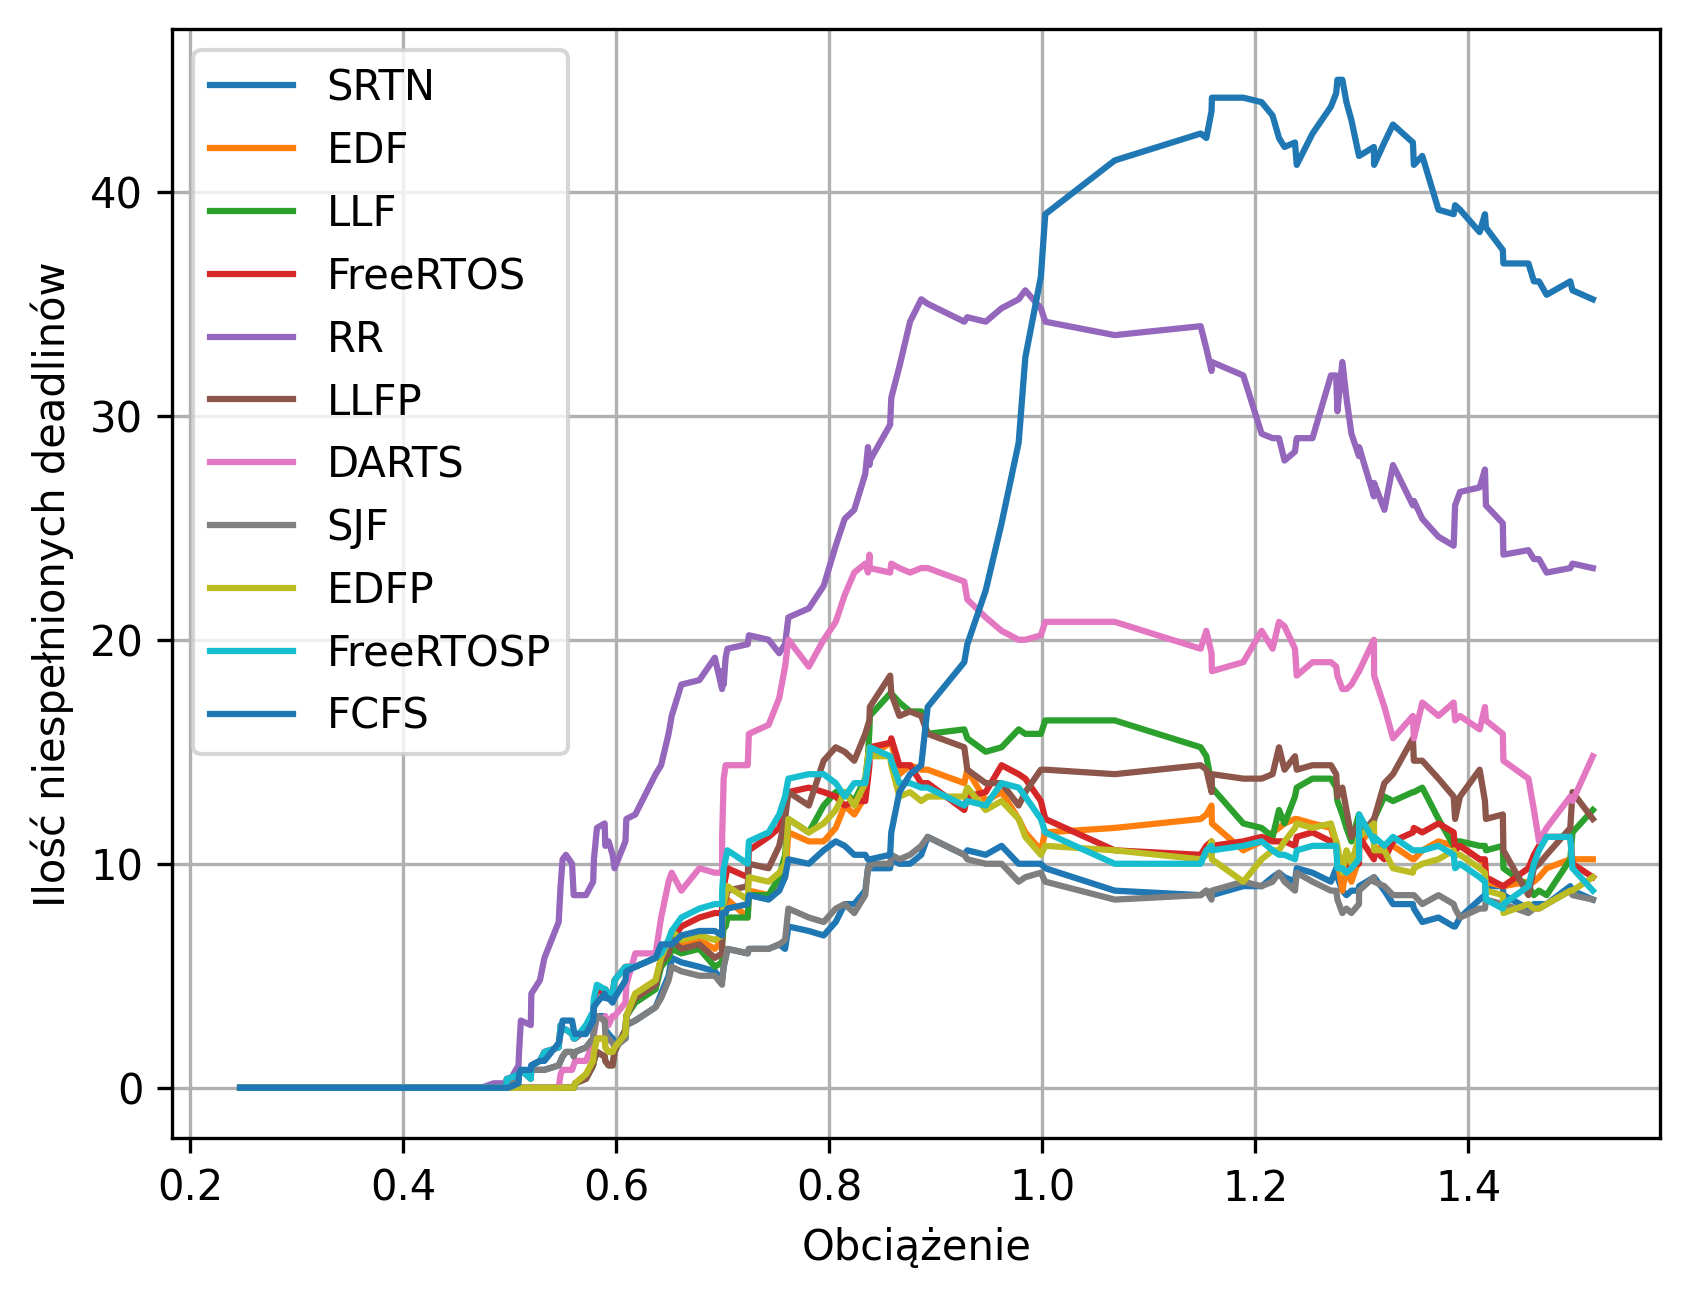
\includegraphics[width=1\textwidth]{Images/diagrams/loadfactor-misses.png}
        \caption{Zależność liczby niespełnionych ograniczeń czasowych od obciążenia systemu}
        \label{fig:loadfactor-misses}
    \end{subfigure}
    \hfill
    \begin{subfigure}{0.85\textwidth}
        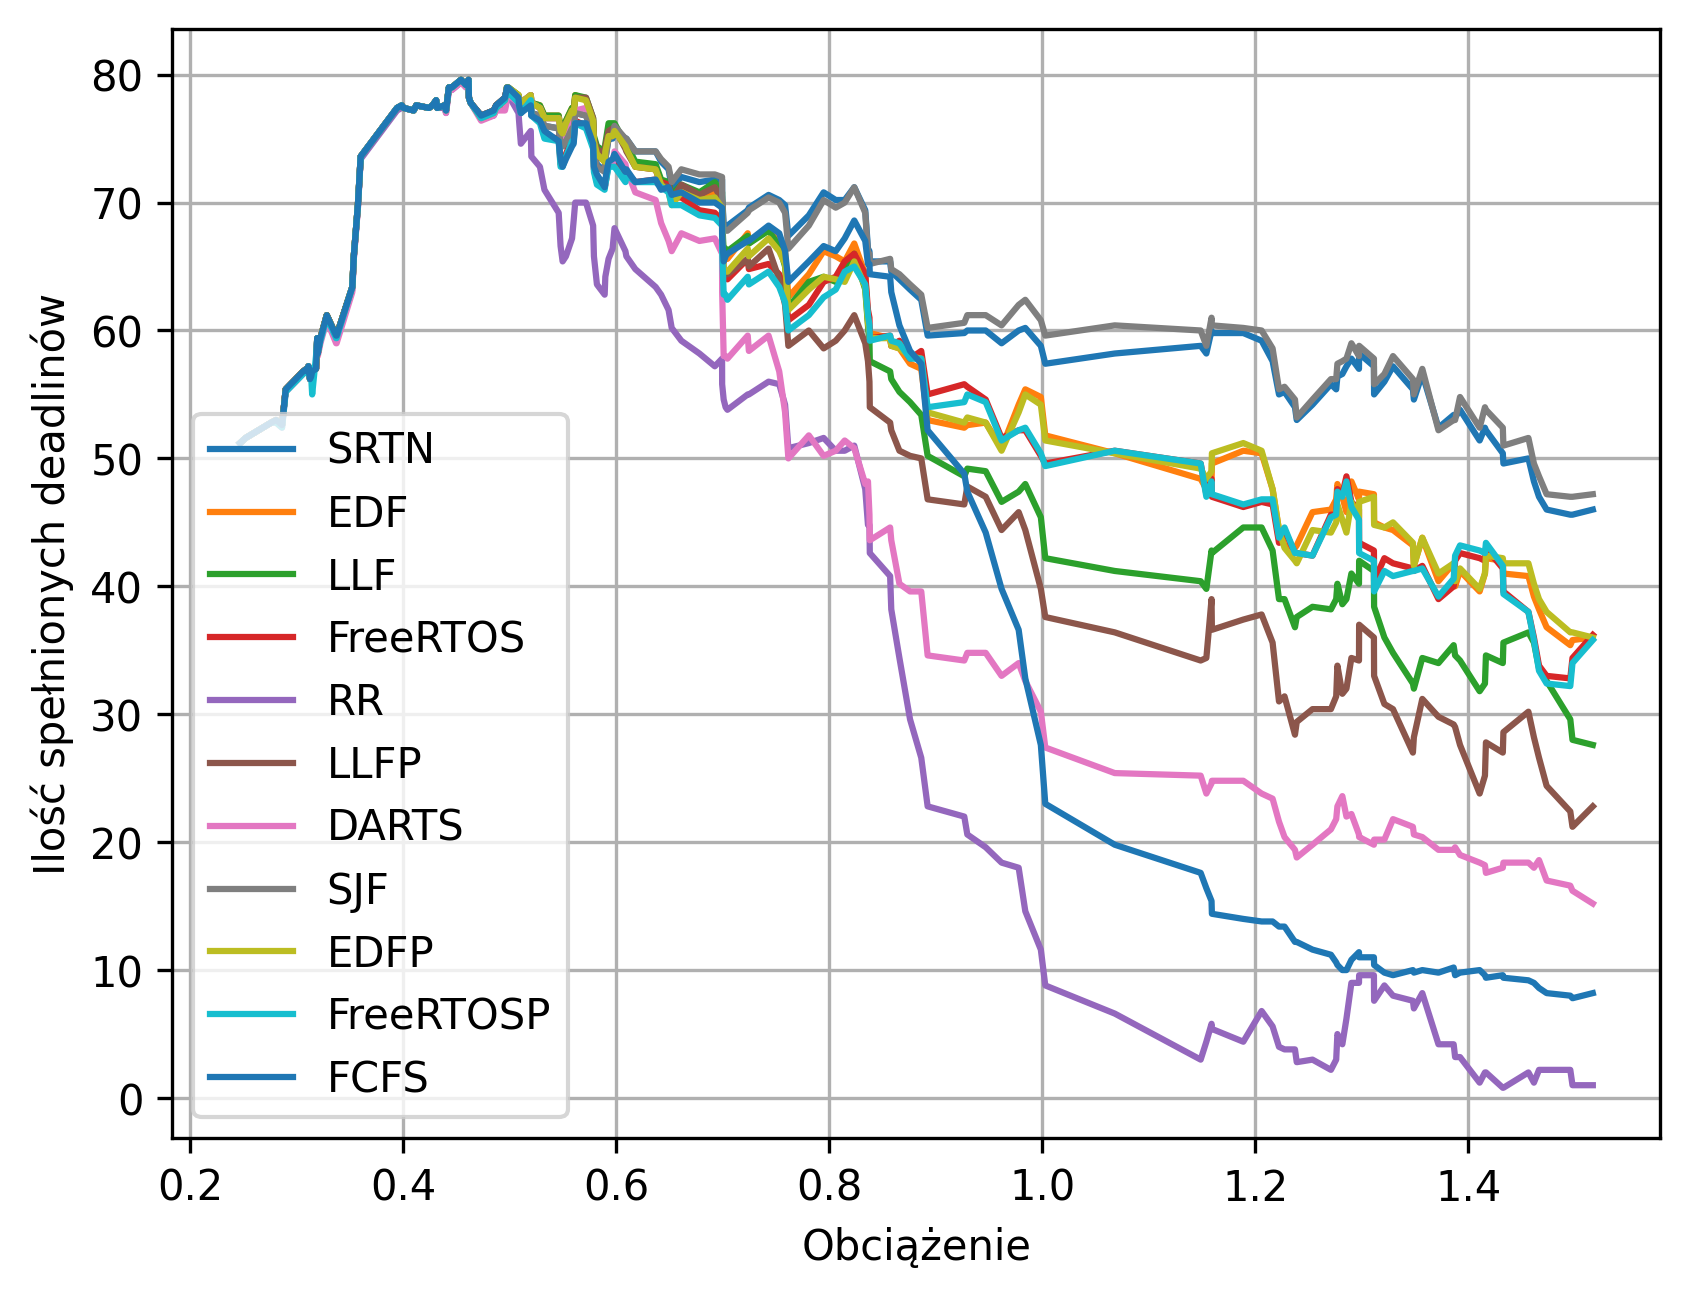
\includegraphics[width=1\textwidth]{Images/diagrams/loadfactor-catches.png}
        \caption{Zależność liczby spełnionych ograniczeń czasowych od obciążenia systemu}
        \label{fig:loadfactor-catches}
    \end{subfigure}
    \caption{Wyniki testów zgładzone, dla obciążenia i najgorszego czasu osiągnięcia celu (deadline na wykresach), dla każdego algorytmu (dodatek \textit{P} oznacza odmianę algorytmu z dodaniem wywłaszczania)}
    \label{fig:results-loadfactor}
\end{figure}

%\begin{figure}[h]
%    \begin{subfigure}[b]{0.9\textwidth}
%        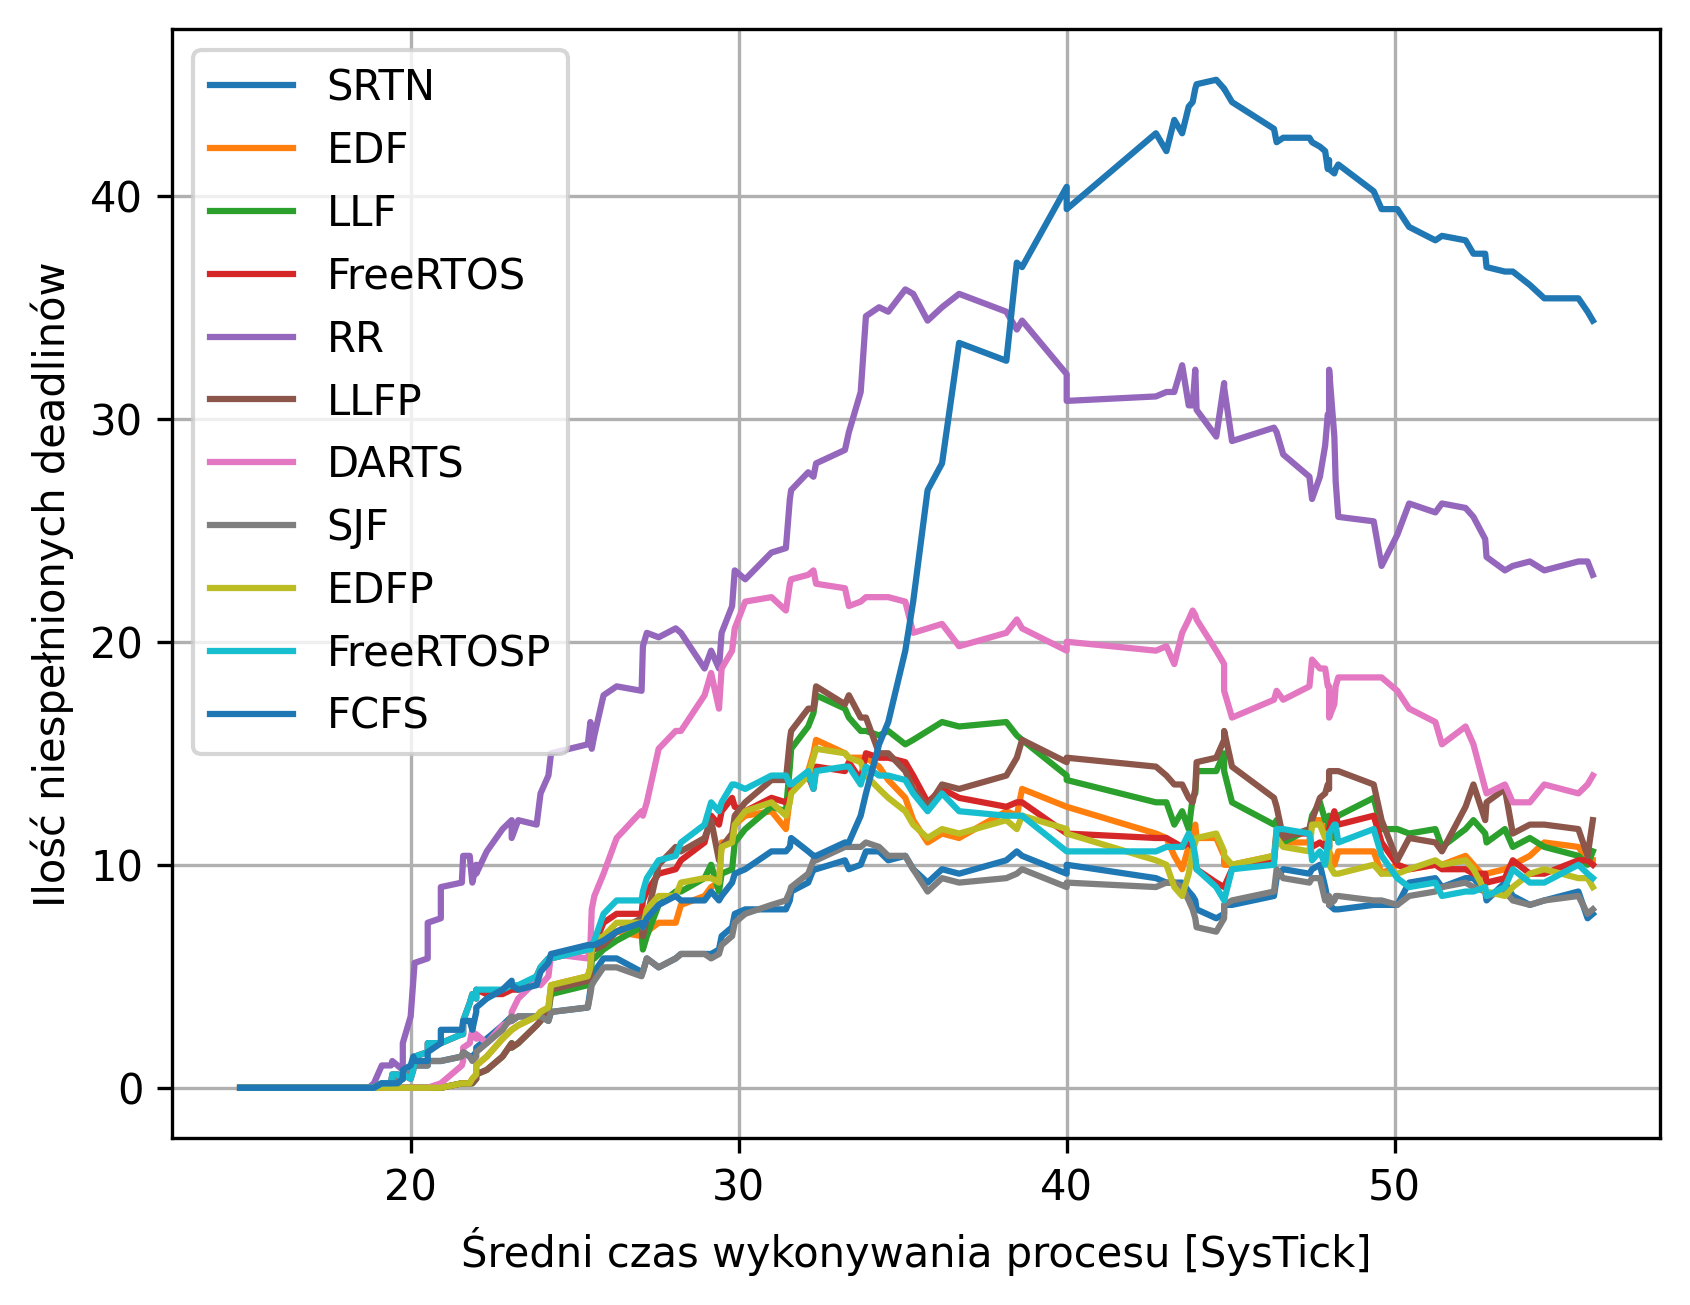
\includegraphics[width=1\textwidth]{Images/diagrams/avaragetime-misses.png}
%        \caption{Zależność ilości niespełnionych ograniczeń czasowych od średniego czasu potrzebnego procesu na osiągnięcie celu}
%        \label{fig:avaragetime-misses}
%    \end{subfigure}
%    \hfill
%    \begin{subfigure}[b]{0.9\textwidth}
%        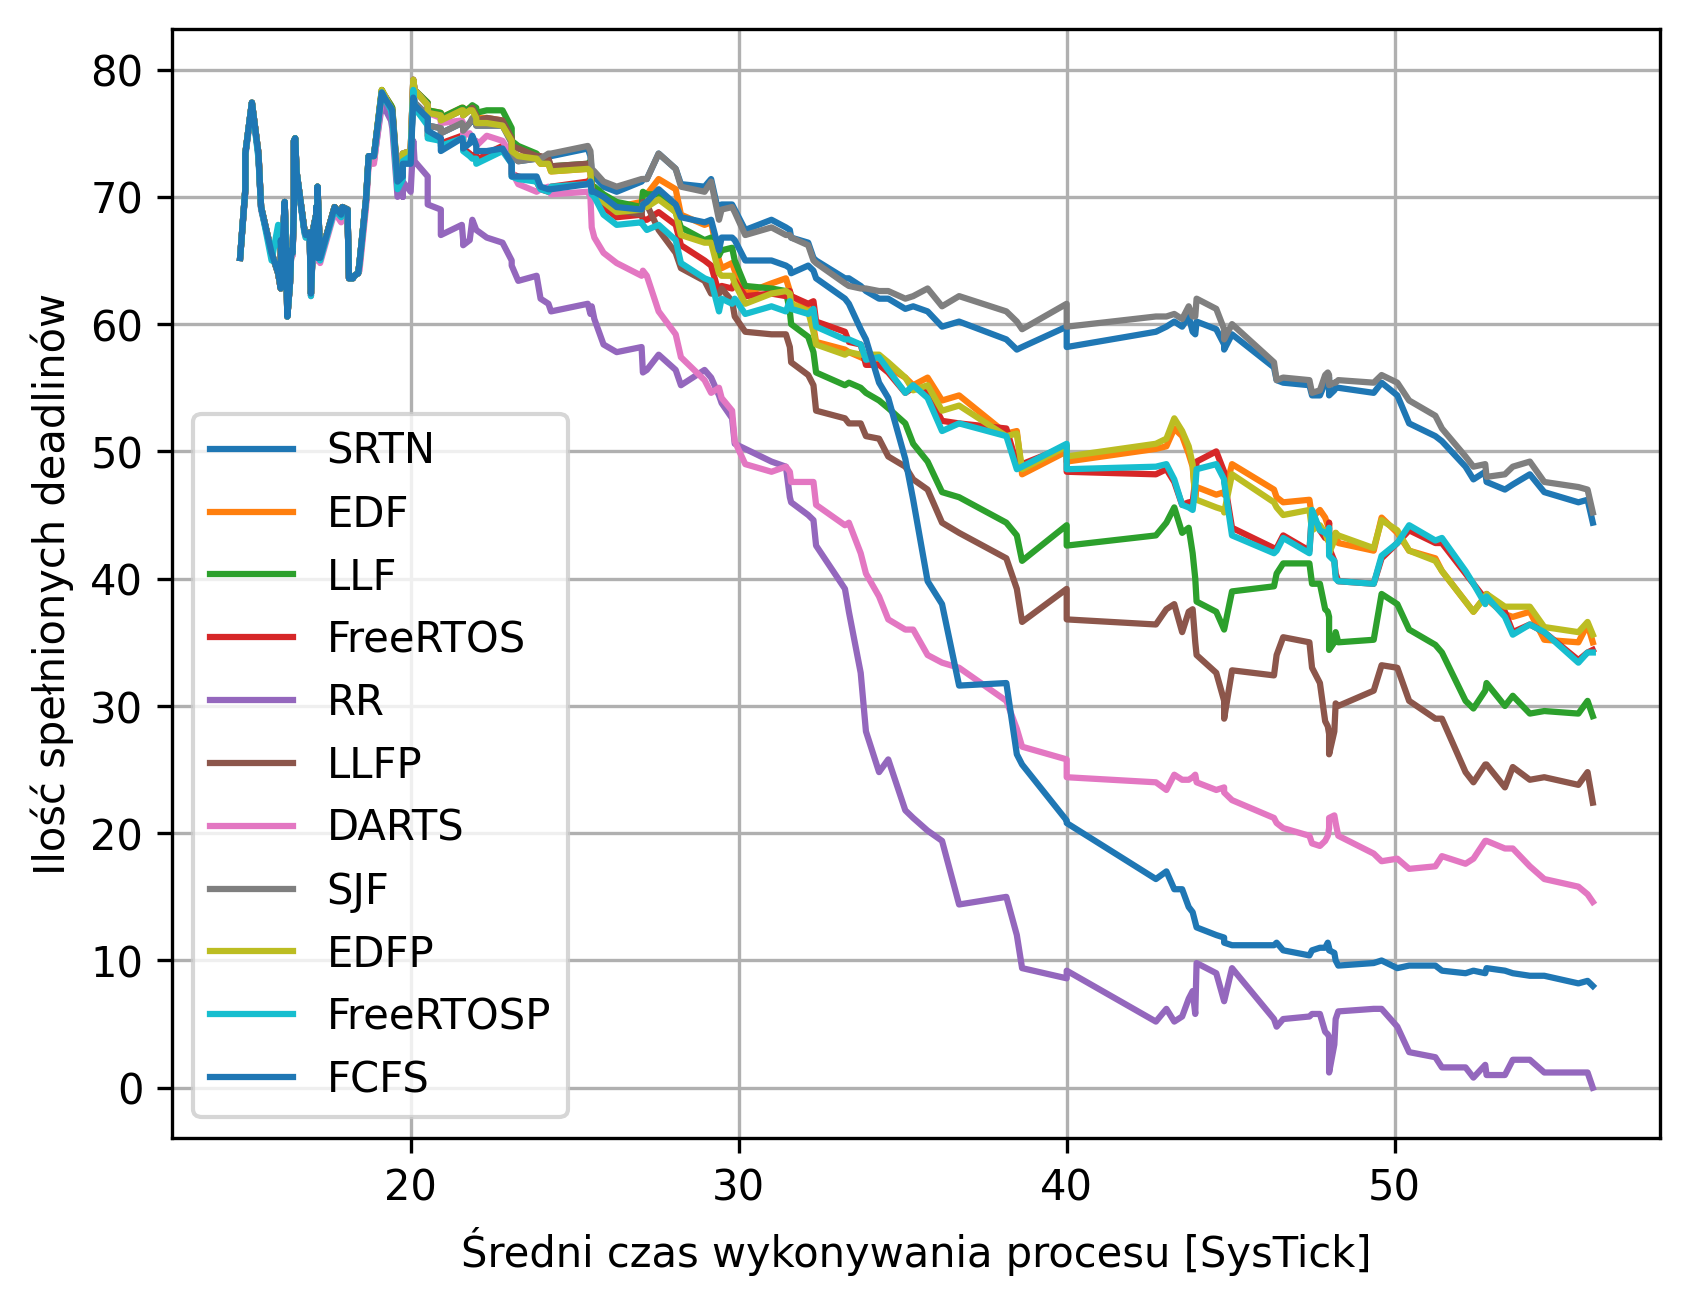
\includegraphics[width=1\textwidth]{Images/diagrams/avaragetime-catches.png}
%        \caption{Zależność ilości spełnionych ograniczeń czasowych od średniego czasu potrzebnego procesu na osiągnięcie celu}
%        \label{fig:avaragetime-catches}
%    \end{subfigure}
%    \caption{Wyniki testów zgładzone, dla średniego czasu wykonywania procesu i najgorszego czasu osiągnięcia celu (deadline na wykresach), dla każdego algorytmu (dodatek \textit{P} oznacza odmianę algorytmu z dodaniem wywłaszczania)}
%    \label{fig:results-avtime}
%\end{figure}

\begin{figure}[h]
    \centering
    \begin{subfigure}{0.85\textwidth}
        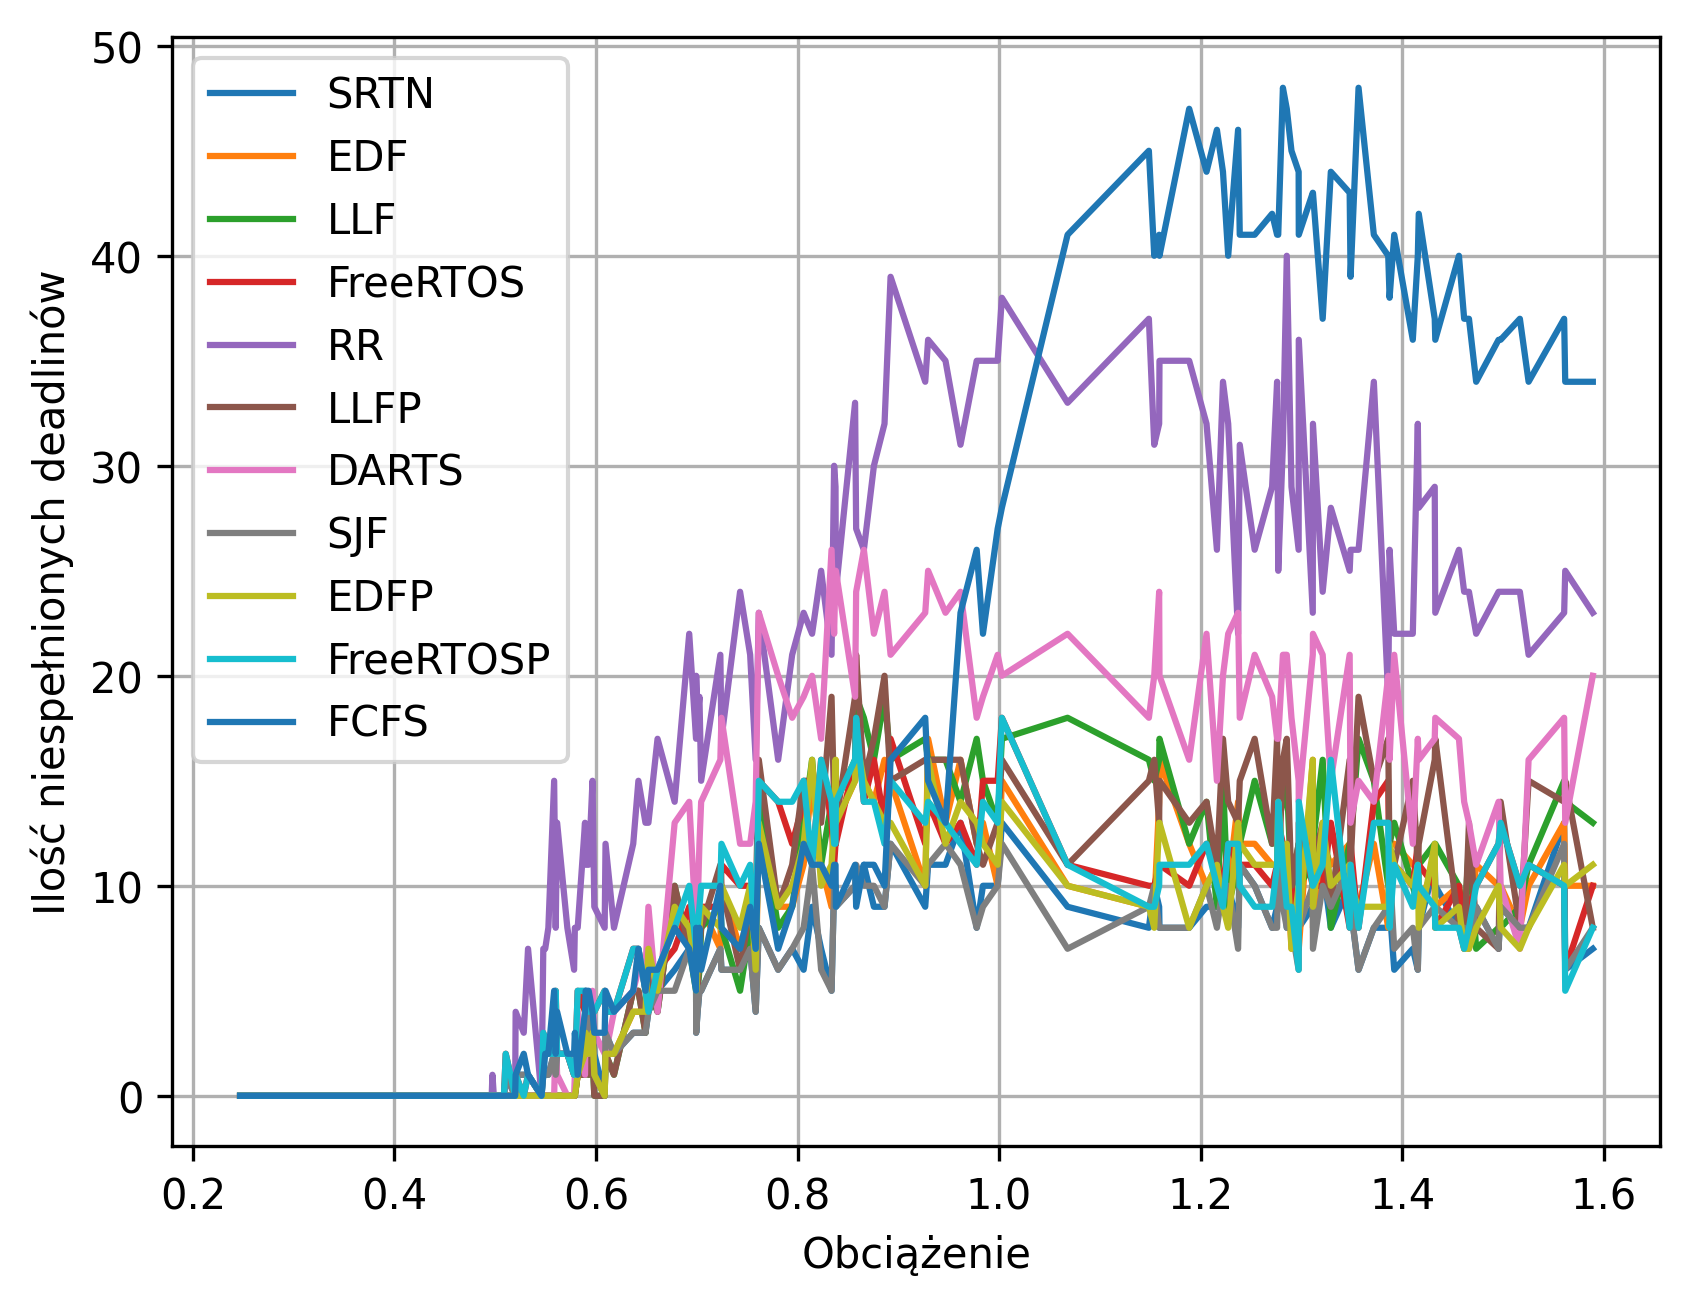
\includegraphics[width=1\textwidth]{Images/diagrams/loadfactor-misses-notsmoothed.png}
        \caption{Zależność liczby niespełnionych ograniczeń czasowych od obciążenia systemu}
        \label{fig:loadfactor-misses-notsmoothed}
    \end{subfigure}
    \hfill
    \begin{subfigure}{1\textwidth}
        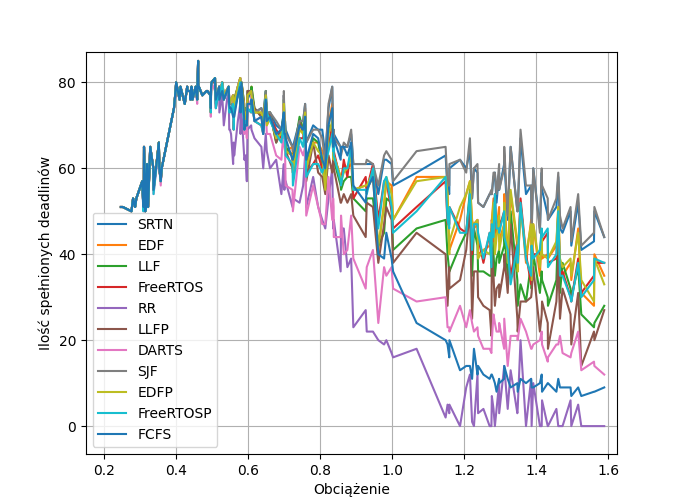
\includegraphics[width=1\textwidth]{Images/diagrams/loadfactor-catches-notsmoothed.png}
        \caption{Zależność liczby spełnionych ograniczeń czasowych od obciążenia systemu}
        \label{fig:loadfactor-catches-notsmoothed}
    \end{subfigure}
    \caption{Wyniki testów nie zgładzone, dla obciążenia i najgorszego czasu osiągnięcia celu (deadline na wykresach), dla każdego algorytmu (dodatek \textit{P} oznacza odmianę algorytmu z dodaniem wywłaszczania)}
    \label{fig:results-notsmoothed-loadfactor}
\end{figure}

%\begin{figure}[h]
%    \begin{subfigure}[b]{0.9\textwidth}
%        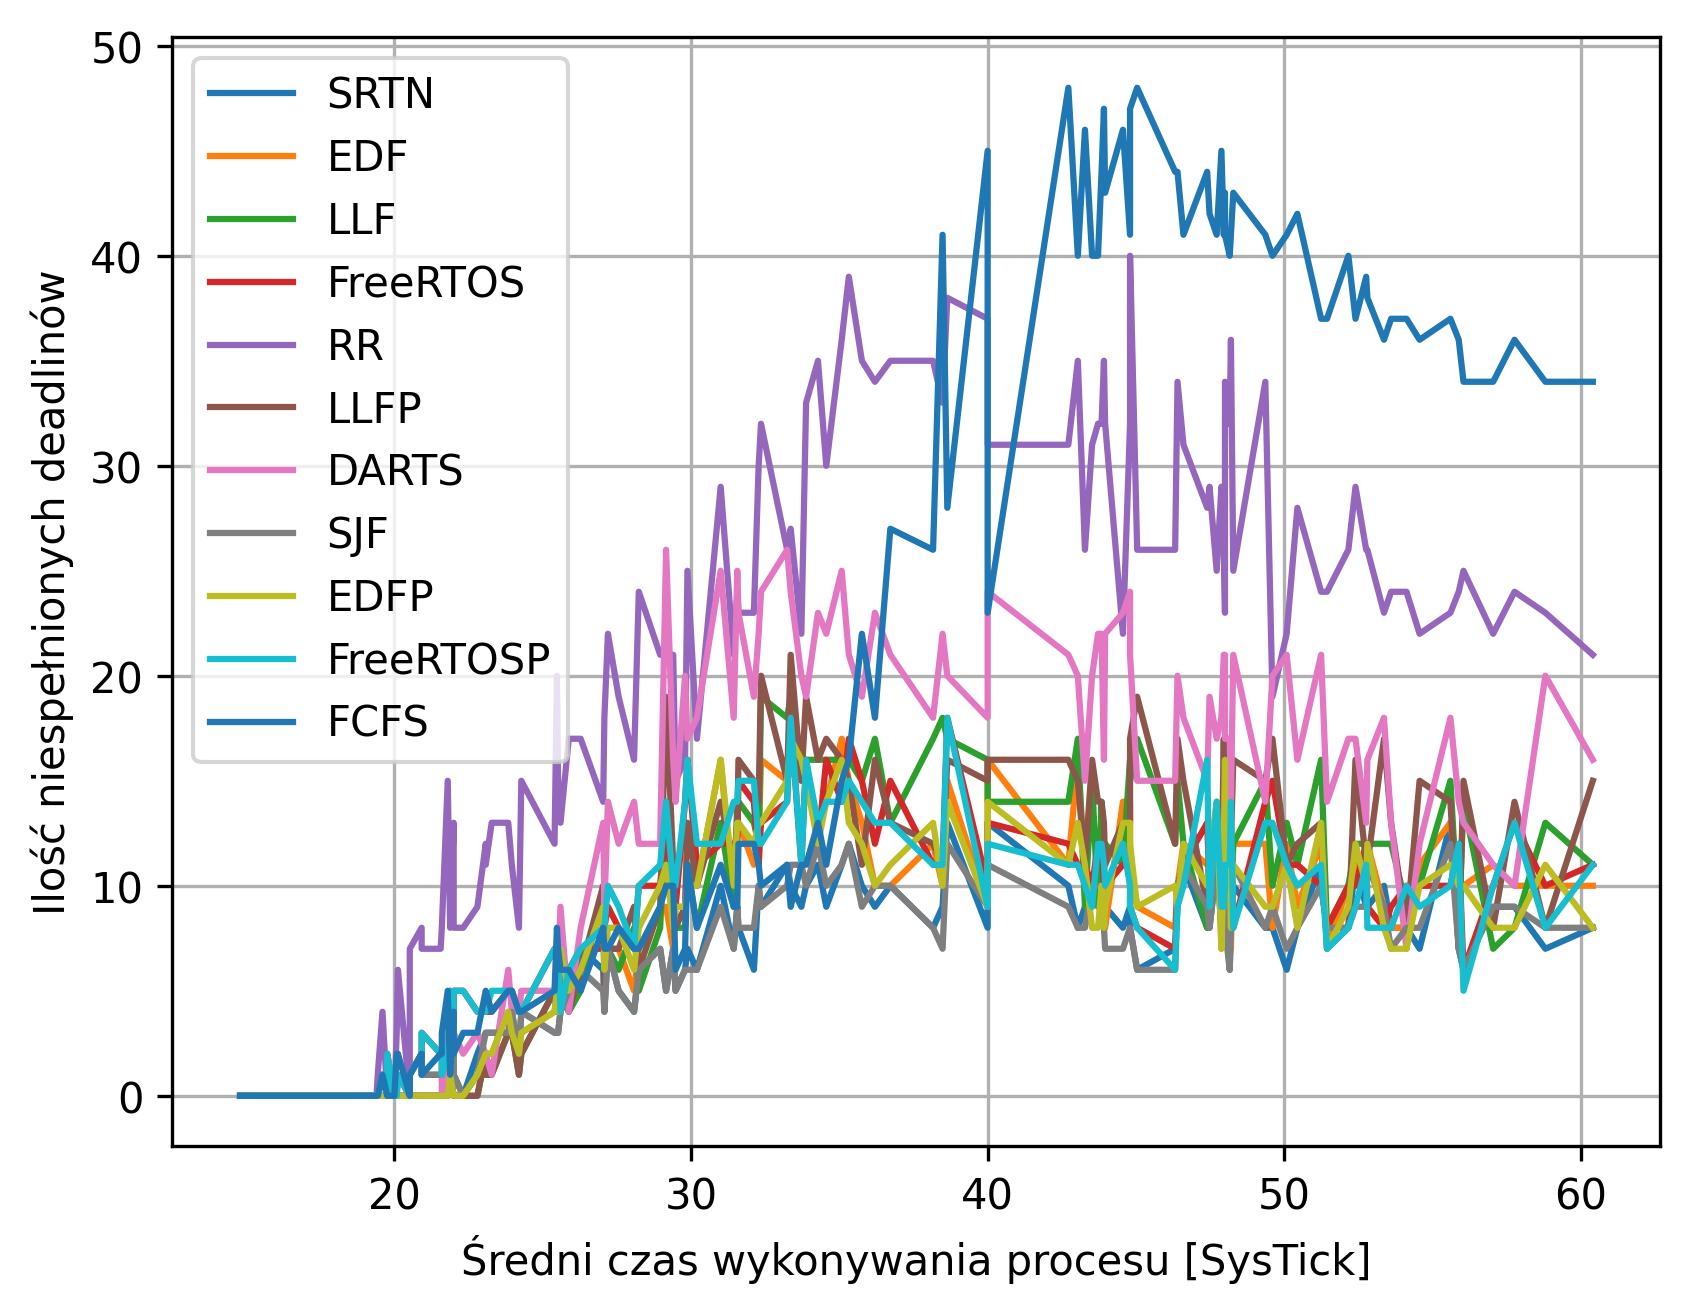
\includegraphics[width=1\textwidth]{Images/diagrams/avaragetime-misses-notsmoothed.png}
%        \caption{Zależność ilości niespełnionych ograniczeń czasowych od średniego czasu potrzebnego procesu na osiągnięcie celu}
%        \label{fig:avaragetime-misses-notsmoothed}
%    \end{subfigure}
%    \hfill
%    \begin{subfigure}[b]{0.9\textwidth}
%        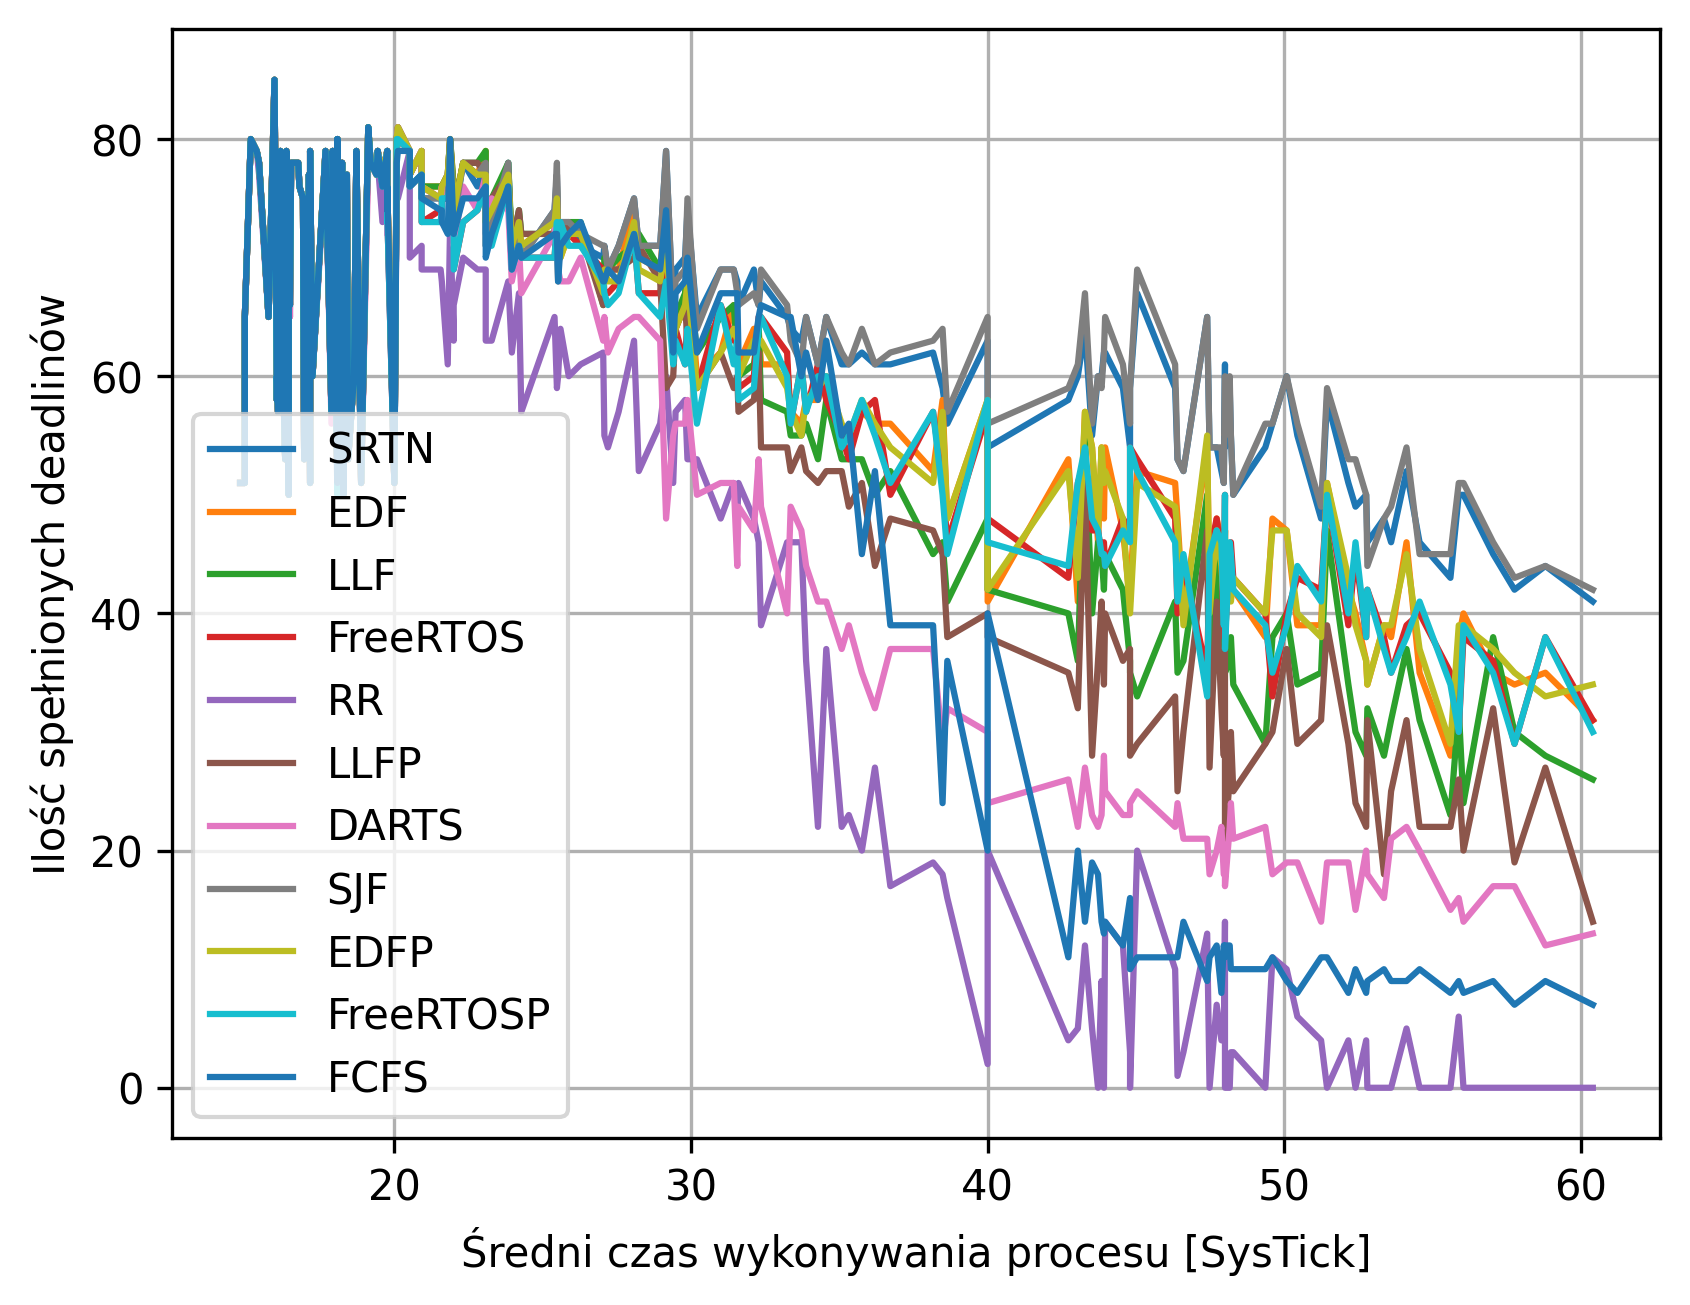
\includegraphics[width=1\textwidth]{Images/diagrams/avaragetime-catches-notsmoothed.png}
%        \caption{Zależność ilości spełnionych ograniczeń czasowych od średniego czasu potrzebnego procesu na osiągnięcie celu}
%        \label{fig:avaragetime-catches-notsmoothed}
%    \end{subfigure}
%    \caption{Wyniki testów nie zgładzone, dla średniego czasu wykonywania procesu i najgorszego czasu osiągnięcia celu (deadline na wykresach), dla każdego algorytmu (dodatek \textit{P} oznacza odmianę algorytmu z dodaniem wywłaszczania)}
%    \label{fig:results-notsmoothed-avtime}
%\end{figure}

Dla porównania zaimplementowanych algorytmów zostało wygenerowano 165 zestawów danych procesów z wartościami obciążenia od $0,246$ do $1,589$. Każdy zbiór zawierał 25 procesów, których metadane zostały wygenerowane losowo, używając rozkładów prawdopodobieństwa (zgodnie z opisem skryptu \textit{generate.py}). Dane dla każdego testu były zbierane do momentu, gdy wartość zegara systemu operacyjnego osiągała 2500 SysTick. Po osiągnięciu tej wartości zegara, narzędzia pomiarowe przechodziły do analizy zebranych danych.

Każdy z zaimplementowanych algorytmów został przetestowany przy użyciu tego zbioru danych. Przetestowane także zostały dwie odmiany standardowego algorytmu FreeRTOS: bez wywłaszczania i współdzielenia, oraz z wywłaszczaniem i bez współdzielenia. Algorytm FreeRTOS'a wymaga wygenerowania priorytetów, więc do wspomnianych wyżej wygenerowanych danych dodano priorytety w zakresie od 1 do 255. Powtarzanie priorytetów było wyłączone.

Wyniki przeprowadzonych testów w wersji graficznej są zamieszczone na \cref{fig:results-notsmoothed-loadfactor}. Po analizie stwierdzono, że w celu porównania rezultatów algorytmów należy wygładzić wyniki, aby pozbyć się niepotrzebnych w tym przypadku wahań. Wahania te będą omówione oddzielnie. Zgładzona wersja wyników w postaci graficznej jest pokazana na \cref{fig:results-notsmoothed-loadfactor}. Dla wygładzania użyto algorytmu Simple Moving Average, który obliczał średnią z 5 punktów.

Analizując dane, można zanotować następujące fakty:

\begin{enumerate}
    \item Wszystkie algorytmy z sukcesem radziły z zarządzaniem systemem do wartości obciążenia $0.496$.
    \item Pierwszym algorytmem, którego procesy zaczęły spóźniać się z osiągnięciem celu jest FCFS.
    \item Najgorzej z wszystkich w zarządzaniu procesami były trzy algorytmy: FCFS, RR i DARTS. Pozostałe radziły z zadaniem w przybliżeniu z tym samym sukcesem.
    \item Najlepiej z zadaniem, szczególnie przy obciążeniu większym niż $0.7$, poradziły algorytmy SJF i SRTN.
    \item Rożnica pomiędzy dwoma przetestowanymi odmianami standardowego algorytmu FreeRTOS jest znikoma, jak również i pomiędzy odmianami LLF i EDF.
\end{enumerate}

Fakt, że DARTS znalazł się wśród najgorszych wyników, był nieoczekiwany, biorąc pod uwagę skomplikowaność algorytmu.

Podczas analizy zauważono jedną niezgodność w wynikach. Patrząc na \cref{fig:loadfactor-misses}, można dostrzec, że w pewnym momencie ilość opóźnień dla każdego algorytmu zaczyna spadać, mimo ciągłego zwiększania obciążenia. Jest to trochę mylące, ponieważ, gdy algorytm przy pewnej wartości obciążenia systemu zaczyna wykazywać wzrost liczby niespełnionych celów w określonych terminach, to przy dalszym zwiększaniu obciążenia, oczekiwany jest dalszy wzrost liczby opóźnień (zakładając, że ilość procesów w systemie się nie zmienia, co jest prawdą w badanym przypadku). Dlaczego więc w tym przypadku wartość opóźnień się zmniejsza?

Aby odpowiedzieć na to pytanie, należy przyjrzeć się wykresowi \cref{fig:loadfactor-catches}, który pokazuje liczbę osiągniętych celów bez opóźnienia. Uwzględniając powyższe, jeśli liczba niespełnionych celów spada, to liczba spełnionych celów, przedstawiona na \cref{fig:loadfactor-catches}, powinna rosnąć. Jednak na \cref{fig:loadfactor-catches}, liczba spełnionych celów ciągle spada. Gdzie są wtedy te spełnione lub niespełnione cele?

Problem był ukryty w sposobie śledzenia wykonywania procesów i dokonywania pomiarów wybranym w ramach tej pracy. Skrypt \textit{parse.py} wykrywa aktywność procesów na podstawie wykonywanych funkcji, które są odpowiednikami procesów w FreeRTOS i są wykonywane tylko wtedy, gdy nadzorca przydzieli im zasoby jednostki obliczeniowej. W przypadku zwiększenia obciążenia systemu, niektóre procesy mogą w ogóle nie dostawać zasobów jednostki obliczeniowej, co uniemożliwia nawet rozpoczęcie wykonywania.

Fakt, że niektóre procesy przy większym obciążeniu nie mogą rozpocząć swojego wykonywania, oraz sam sposób wykrywania aktywności procesów, prowadzą do wniosku, że sukcesy lub porażki w osiągnięciu celów nie zostały wykryte, ponieważ procesy te nawet nie zaczęły swoje wykonywanie. To z kolei spowodowało ich niewykrycie podczas pomiarów i analizy. Skoro te procesy nawet nie rozpoczęły swojego wykonywania, można je przepisać do grupy procesów, którym nie udało się osiągnąć swojego celu w wyznaczonych ograniczeniach czasowych. Taki stan można nazwać nasyceniem.

\FloatBarrier

Patrząc na wyniki, można też zauważyć, że algorytmy SRTN i SJF zachowują się najlepiej w tym stanie.

Jeżeli chodzi o niewygładzone wyniki, głównym pytaniem jest, dlaczego te wyniki charakteryzują się tak dużymi wahaniami wartości spełnionych i niespełnionych celów w ramach ograniczeń czasowych? Odpowiedź jest ukryta w generacji danych dla testów.

Jak było wspomniane przy opisie skryptu \textit{generate.py} (przykład \ref{lst:proces-parameters-generated}), proces posiada listę metadanych, która nie ogranicza się tylko i wyłącznie obciążeniem systemu, które jest relacją pomiędzy czasem potrzebnym na osiągnięcie celu, okresem przejścia procesu do stanu gotowości i liczbą procesów zdefiniowaną statycznie (zgodnie z formułą \cref{eq:utilization}). To właśnie te metadane, a dokładnie ich wzajemna relacja, stanowią drugi najważniejszy czynnik (obok używanego algorytmu do zarządzania zasobami jednostki obliczeniowej) wpływający na ostateczny wynik.

Fakt, że wszystkie metadane procesów były generowane losowo, uwzględniając tylko jedną zależność pomiędzy trzema zmiennymi, spowodował takie wahania w finalnych rezultatach.

\end{document}